\documentclass[12pt, a4paper]{report}

% --- Packages ---
\usepackage[utf8]{inputenc}
\usepackage[T1]{fontenc}
\usepackage[french]{babel}
\usepackage{graphicx}
\usepackage{booktabs}
\usepackage{amsmath}
\usepackage{geometry}
\usepackage{array}
\usepackage{enumitem}
\usepackage{hyperref}
\usepackage{xcolor}
\usepackage{titlesec}
\usepackage{lmodern}
\usepackage{microtype}
\usepackage{fancyhdr}
\usepackage{listings}
\usepackage[scaled=0.85]{beramono}

% --- Font Configuration ---

% --- Color Definitions ---
\definecolor{primary}{RGB}{0,51,102}
\definecolor{secondary}{RGB}{102,102,153}
\definecolor{accent}{RGB}{204,0,0}
\definecolor{codegray}{rgb}{0.5,0.5,0.5}
\definecolor{codepurple}{rgb}{0.58,0,0.82}
\definecolor{codeblue}{rgb}{0,0,0.9}
\definecolor{codegreen}{rgb}{0.1,0.6,0.1}

% --- Page Geometry ---
\geometry{
  a4paper,
  left=2.5cm,
  right=2.5cm,
  top=2.5cm,
  bottom=2.5cm,
  headheight=15pt
}

% --- Header/Footer Setup ---
\pagestyle{fancy}
\fancyhf{}
\fancyhead[L]{\small Rapport de Stage}
\fancyhead[R]{\small Zakaria el Khaldi}
\fancyfoot[C]{\thepage}
\renewcommand{\headrulewidth}{0.4pt}
\renewcommand{\footrulewidth}{0.4pt}

% --- Title Formatting ---
\titleformat{\chapter}
  {\normalfont\LARGE\bfseries\color{primary}}
  {\thechapter}{1em}{}
\titleformat{\section}
  {\normalfont\Large\bfseries\color{primary}}
  {\thesection}{1em}{}
\titleformat{\subsection}
  {\normalfont\large\bfseries\color{secondary}}
  {\thesubsection}{1em}{}
\titleformat{\subsubsection}
  {\normalfont\normalsize\bfseries\color{accent}}
  {\thesubsubsection}{1em}{}

% --- List Formatting ---
\setlist[itemize]{leftmargin=*, nosep}
\setlist[enumerate]{leftmargin=*, nosep}

% --- Hyperlink Setup ---
\hypersetup{
  colorlinks=true,
  linkcolor=primary,
  urlcolor=secondary,
  citecolor=accent
}

% --- Listings Setup for Code ---
\lstdefinestyle{codestyle}{
    basicstyle=\ttfamily\footnotesize,
    numbers=left,
    numberstyle=\tiny\color{codegray},
    stepnumber=1,
    numbersep=5pt,
    backgroundcolor=\color{white!95!black},
    showspaces=false,
    showstringspaces=false,
    showtabs=false,
    frame=tb,
    framextopmargin=3pt,
    framexbottommargin=3pt,
    rulecolor=\color{black!30!white},
    tabsize=2,
    captionpos=b,
    breaklines=true,
    breakatwhitespace=false,
    stringstyle=\color{codepurple},
    commentstyle=\color{codegreen},
    keywordstyle=\color{codeblue}
}

% --- Image path configuration ---
% When you upload images to Overleaf, place them in folders named:
% week_1_img, week_2_img, week_3_img, week_4_img
\graphicspath{{week_1_img/}{week_2_img/}{week_3_img/}{week_4_img/}}

% --- Document Information ---
\title{\Huge\bfseries\color{primary} Rapport de Stage \\ 
       \Large Conception et Développement d'une Plateforme E-learning}
\author{\Large Zakaria el Khaldi}
\date{\large Juin 2025}

\begin{document}

% --- Cover Page ---
\begin{titlepage}
  \centering
  \IfFileExists{images/logo_entreprise.png}{
    \includegraphics[width=0.4\textwidth]{images/logo_entreprise.png}
  }{
    % If logo doesn't exist, display company name in large text
    \vspace*{1cm}
    {\huge\bfseries\color{primary} ENTREPRISE DE STAGE\par}
  }
  \vspace*{2cm}
  
  {\Huge\bfseries\color{primary} RAPPORT DE STAGE\par}
  \vspace{1.5cm}
  {\Large\itshape Conception et Développement d'une Plateforme E-learning\par}
  \vspace{3cm}
  
  {\large Présenté par :\par}
  \vspace{0.5cm}
  {\Large\bfseries Zakaria el Khaldi\par}
  \vspace{1.5cm}
  
  {\large Stage effectué du 10 mai au 10 juin 2025\par}
  \vspace{0.5cm}
  {\large Au sein de l'entreprise :\par}
  \vspace{0.5cm}
  {\large\bfseries LearnTech Solutions\par}
  \vspace{3cm}
  
  {\large Sous la supervision de :\par}
  \vspace{0.5cm}
  {\large M. Ahmed Benali\par}
  \vspace{0.5cm}
  {\large Directeur Technique\par}
  \vfill
  
  {\large\bfseries Formation : Master en Développement Informatique\par}
  \vspace{0.5cm}
  {\large Année Académique 2024-2025\par}
\end{titlepage}

% --- Remerciements ---
\chapter*{Remerciements}
\addcontentsline{toc}{chapter}{Remerciements}
\thispagestyle{fancy}

Je tiens à exprimer ma profonde gratitude à toutes les personnes qui ont contribué à la réussite de ce stage et à l'élaboration de ce rapport.

Je remercie tout d'abord M. Ahmed Benali, Directeur Technique de LearnTech Solutions, pour son accueil au sein de l'entreprise, sa disponibilité et ses précieux conseils qui m'ont guidé tout au long de cette expérience professionnelle.

Mes remerciements s'adressent également à l'ensemble de l'équipe de LearnTech Solutions pour leur accueil chaleureux, leur soutien et leur partage de connaissances qui ont rendu cette expérience particulièrement enrichissante.

Je suis également reconnaissant envers mon université et mes professeurs pour la qualité de l'enseignement reçu qui m'a permis d'aborder ce stage avec les compétences nécessaires.

Enfin, je remercie ma famille et mes amis pour leur soutien inconditionnel tout au long de mon parcours.

\newpage

% --- Table of Contents ---
\tableofcontents
\thispagestyle{fancy}
\newpage

\chapter{Introduction}
\thispagestyle{fancy}

Ce rapport présente le travail réalisé lors de mon stage de fin d'études effectué au sein de LearnTech Solutions du 10 mai au 10 juin 2025. Durant cette période, j'ai participé à la conception et au développement d'une plateforme e-learning complète destinée aux entreprises et aux professionnels individuels.

L'objectif de ce stage était de mettre en pratique les connaissances théoriques acquises durant ma formation et de les approfondir dans un contexte professionnel. Ce projet m'a permis de développer des compétences en développement web, en conception d'architecture logicielle, en gestion de bases de données et en traitement de données.

Ce rapport détaille l'ensemble des travaux réalisés durant les différentes semaines du stage, les méthodologies employées, les difficultés rencontrées et les solutions apportées, ainsi que les résultats obtenus.

\section{Contexte du Stage}
LearnTech Solutions est une entreprise spécialisée dans le développement de solutions d'apprentissage en ligne. Face à une demande croissante pour des plateformes de formation à distance, l'entreprise a décidé de développer une nouvelle plateforme e-learning innovante combinant des cours structurés et des services de consultation personnalisés.

Le projet s'inscrit dans un contexte de digitalisation accélérée de la formation professionnelle et de besoin croissant en solutions permettant un apprentissage flexible et adapté aux besoins spécifiques des entreprises et des individus.

\section{Présentation de l'Entreprise}
LearnTech Solutions est une entreprise tech spécialisée dans le développement de solutions éducatives numériques. Fondée en 2020, elle se positionne comme un acteur innovant dans le domaine de l'e-learning et des technologies éducatives. L'entreprise compte une vingtaine de collaborateurs, principalement des développeurs, des designers UX/UI, des spécialistes en contenu pédagogique et des experts en expérience utilisateur.

La mission de LearnTech Solutions est de démocratiser l'accès à une éducation de qualité grâce à des plateformes technologiques avancées et intuitives. L'entreprise se distingue par son approche qui combine apprentissage structuré et interaction humaine à la demande.

\section{Objectifs du Stage}
Les objectifs principaux de ce stage étaient les suivants :

\begin{itemize}
  \item Participer à la conception initiale de l'architecture de la plateforme e-learning
  \item Développer des composants back-end pour la gestion des utilisateurs et des cours
  \item Mettre en place un système de traitement et de nettoyage de données pour les contenus pédagogiques
  \item Implémenter des fonctionnalités front-end pour l'expérience utilisateur
  \item Contribuer à l'intégration des différents services et microservices
  \item Participer aux phases de test et d'évaluation de la plateforme
\end{itemize}

Ces objectifs s'inscrivent dans le cadre plus large du développement d'une plateforme e-learning complète et innovante, destinée à être commercialisée auprès d'entreprises et de professionnels individuels.

% --- Include Week Files ---
% Each week's content is in a separate file for better organization

% Week 1 content
\chapter{Semaine 1 : Conception et Architecture de la Plateforme E-learning}
\thispagestyle{fancy}

La première semaine du stage a été consacrée à la conception initiale du projet, à la définition de l'architecture backend et des bases de données, ainsi qu'à la création des premiers diagrammes UML.

\section{Vision de la Plateforme}
La phase initiale de conception s'est concentrée sur la définition de la vision, des offres, des utilisateurs cibles et de la valeur unique de la plateforme.

\subsection{Idée Principale et Offres}
La plateforme e-learning conçue repose sur une vision claire :
\begin{itemize}
  \item \textbf{Idée Principale :} Une plateforme e-learning complète pour les entreprises et les professionnels individuels.
  \item \textbf{Offres Clés :}
    \begin{itemize}
      \item Cours en ligne auto-rythmés (vidéos, images, quiz)
      \item Services de support, de conseil et de prestation via une plateforme de réunion personnalisée intégrée
    \end{itemize}
  \item \textbf{Utilisateurs Cibles :} Entreprises (pour la formation des employés) et apprenants individuels (pour l'amélioration des compétences)
  \item \textbf{Valeur Unique :} Un mélange harmonieux d'apprentissage structuré et d'interaction avec des experts à la demande
\end{itemize}

\subsection{Acteurs Utilisateurs Clés}
Les principaux types d'utilisateurs identifiés pour la plateforme sont :
\begin{itemize}
  \item \textbf{Apprenant Individuel :} S'inscrit, s'abonne, apprend, demande des consultations
  \item \textbf{Employé d'Entreprise :} Apprend via l'abonnement de l'entreprise, demande des consultations
  \item \textbf{Administrateur/Manager d'Entreprise :} Gère le compte de l'entreprise, les employés, les abonnements, attribue les cours, consulte les analyses
  \item \textbf{Créateur de Cours :} Conçoit et élabore le contenu des cours (modules, leçons, quiz)
  \item \textbf{Consultant/Fournisseur de Prestations :} Gère sa disponibilité, anime les sessions via la plateforme de réunion
  \item \textbf{Agent de Support Plateforme :} Assiste les utilisateurs pour les problèmes liés à la plateforme et les questions-réponses
  \item \textbf{Administrateur de la Plateforme :} Supervise l'ensemble de la plateforme, les utilisateurs, le contenu, les paramètres
\end{itemize}

\subsection{Fonctionnalités Principales}
Les fonctionnalités essentielles se divisent en trois catégories :
\begin{itemize}
    \item \textbf{E-Learning :}
    \begin{itemize}
        \item Catalogue de cours (filtrable, consultable)
        \item Modules, Leçons (vidéo, basées sur des images)
        \item Quiz et Évaluations
        \item Suivi de la Progression
        \item Certificats de Réussite
        \item Support Multilingue (EN/FR)
        \item Paramètres Utilisateur et Entreprise
    \end{itemize}
    \item \textbf{Consultation et Prestation :}
    \begin{itemize}
        \item Navigation des services
        \item Profils des consultants et disponibilité
        \item Système de réservation/demande
        \item Intégration API avec la plateforme de réunion personnalisée
        \item Facturation des sessions
    \end{itemize}
    \item \textbf{Monétisation :}
    \begin{itemize}
        \item Abonnements pour utilisateurs individuels (accès illimité)
        \item Abonnements pour entreprises (par utilisateur)
        \item Réductions et Démos
    \end{itemize}
\end{itemize}

\section{Diagrammes UML}
La modélisation UML a permis de formaliser la structure et les relations entre les différentes entités du système.

\subsection{Diagramme de Classes}
Le diagramme de classes a été élaboré pour représenter les principales entités du système et leurs relations.

\begin{figure}[h!]
  \centering
  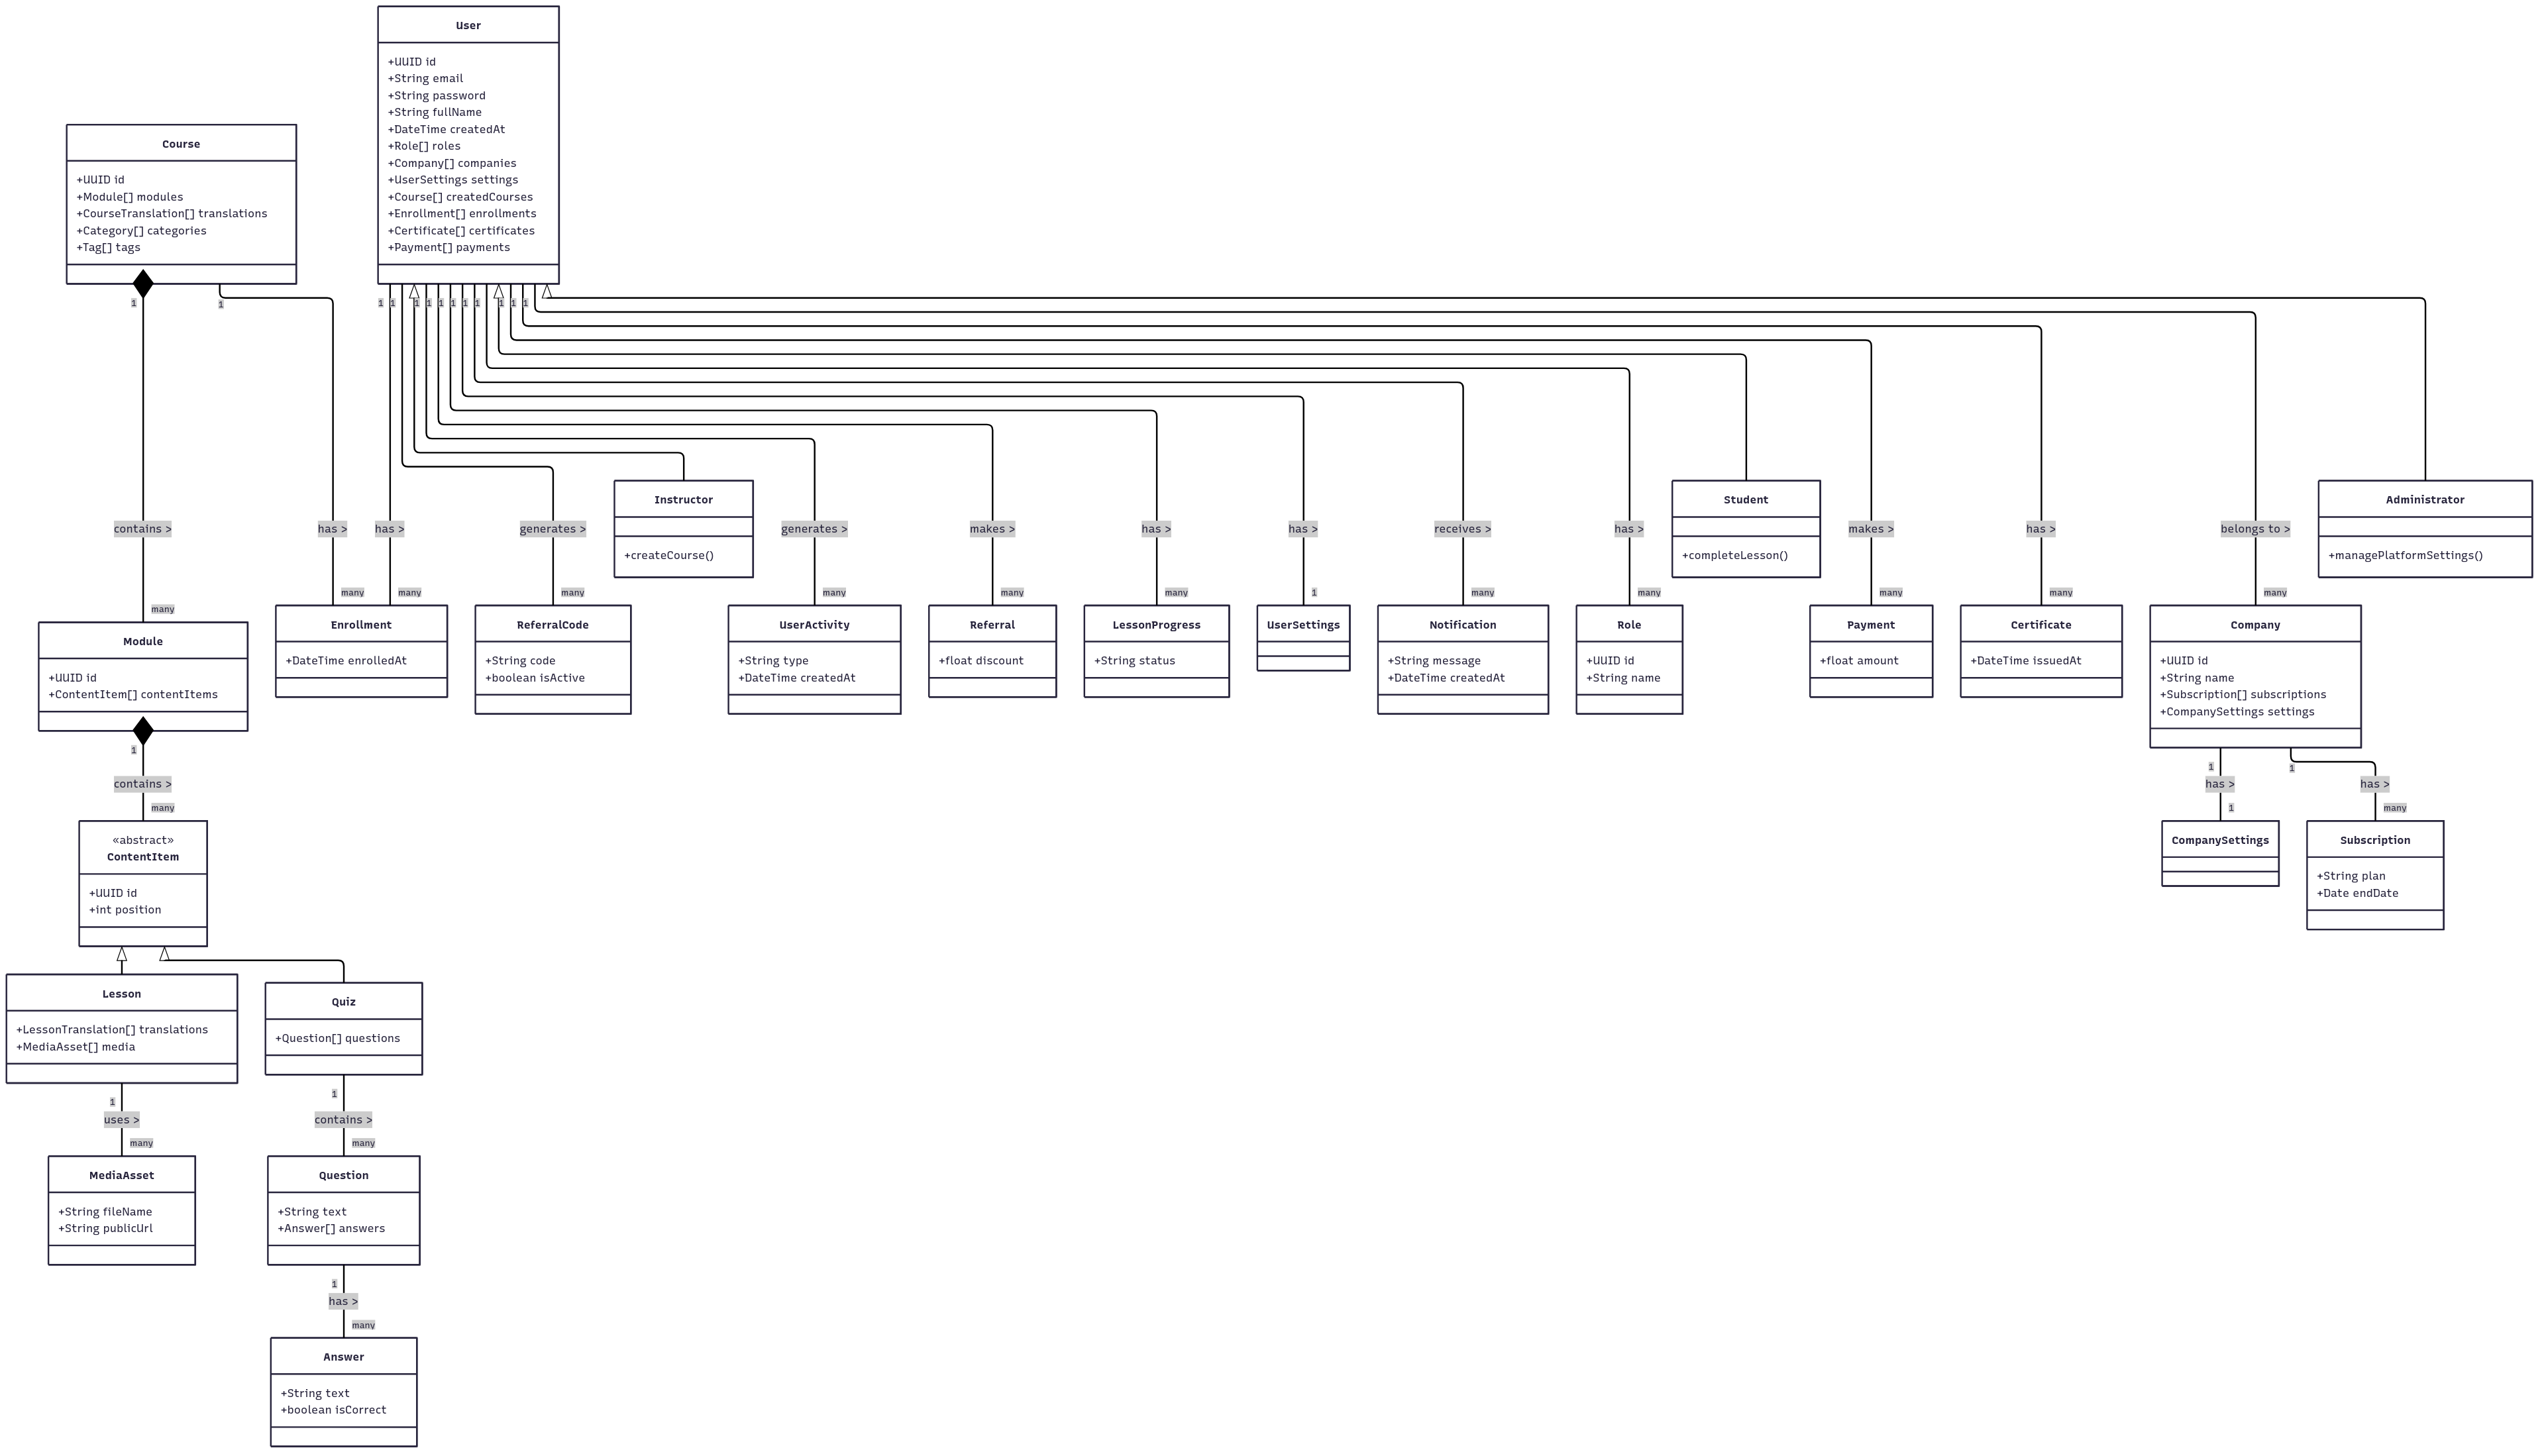
\includegraphics[width=0.9\textwidth,keepaspectratio]{class_diagrame.png}
  \caption{\textbf{Diagramme de classes} de la plateforme e-learning montrant les principales entités et leurs relations.}
  \label{fig:class_diagram}
\end{figure}

Ce diagramme de classes illustre les relations entre les différentes entités du système, comme les utilisateurs, les cours, les modules, les leçons, les abonnements et les services de consultation. Les cardinalités et les types de relations (composition, agrégation, héritage) ont été définies pour refléter précisément la structure du modèle de données.

\section{Architecture Backend et Base de Données}

\subsection{Choix de l'Architecture Microservices}
L'architecture envisagée pour la plateforme repose sur une approche de microservices, justifiée par plusieurs avantages clés :
\begin{itemize}
  \item \textbf{Scalabilité :} Mise à l'échelle indépendante des services individuels selon les besoins
  \item \textbf{Maintenabilité :} Possibilité de modifier des parties spécifiques sans impacter l'ensemble du système
  \item \textbf{Résilience :} Limitation de l'impact des défaillances à des services spécifiques
  \item \textbf{Autonomie des Équipes :} Développement, tests et déploiement indépendants par différentes équipes
  \item \textbf{Flexibilité Technologique :} Utilisation des technologies les plus adaptées pour chaque service
\end{itemize}

\subsection{Pile Technologique}
La pile technologique définie pour le développement comprend :
\begin{itemize}
  \item \textbf{Frontend :} Next.js (React)
  \item \textbf{Microservices Backend :}
    \begin{itemize}
      \item Go (pour les services critiques en performance et concurrents comme les Notifications, le backend de la plateforme de réunion)
      \item Python avec FastAPI (pour les services gourmands en données, développement rapide d'API, par exemple, Catalogue de Cours, Facturation)
      \item Node.js avec Express (TypeScript) (pour les opérations I/O intensives, interaction Supabase, par exemple, IAM, Gestion des Médias)
    \end{itemize}
  \item \textbf{Bases de Données :}
    \begin{itemize}
      \item PostgreSQL (stockage relationnel principal pour la plupart des services)
      \item Supabase (pour l'Authentification, le Stockage, et son Postgres géré pour des services spécifiques)
    \end{itemize}
  \item \textbf{Passerelle API :} Nginx (en tant que reverse proxy et passerelle)
  \item \textbf{Broker de Messages :} Apache Kafka (pour une gestion d'événements asynchrones robuste et scalable)
  \item \textbf{Conteneurisation et Orchestration :} Docker (Kubernetes serait une étape logique suivante pour l'orchestration)
\end{itemize}

\subsection{Architecture Microservices Proposée}
Une décomposition en microservices a été proposée pour répondre aux besoins fonctionnels de la plateforme :
\begin{itemize}
  \item \textbf{Service IAM :} Comptes utilisateurs, rôles, entreprises (Supabase Auth + Node.js/Go)
  \item \textbf{Service Catalogue de Cours :} Structure des cours, métadonnées du contenu (Python/FastAPI + PostgreSQL)
  \item \textbf{Service de Progression de l'Apprenant :} Inscriptions, progression des leçons/quiz, certificats (Python/FastAPI ou Go + PostgreSQL)
  \item \textbf{Service de Réservation :} Demandes de consultation, planification (Node.js/Python + PostgreSQL)
  \item \textbf{Service de Facturation :} Abonnements, paiements, factures (Python/FastAPI + PostgreSQL)
  \item \textbf{Service Média :} Téléchargements de vidéos/images et métadonnées (Supabase Storage + Node.js/Go)
  \item \textbf{Service de Notification :} Envoi d'emails, notifications in-app (Go/Node.js + Kafka)
  \item \textbf{Autres services :} Feedback, Configuration Plateforme, Analytics, etc.
\end{itemize}

\begin{figure}[h!]
  \centering
  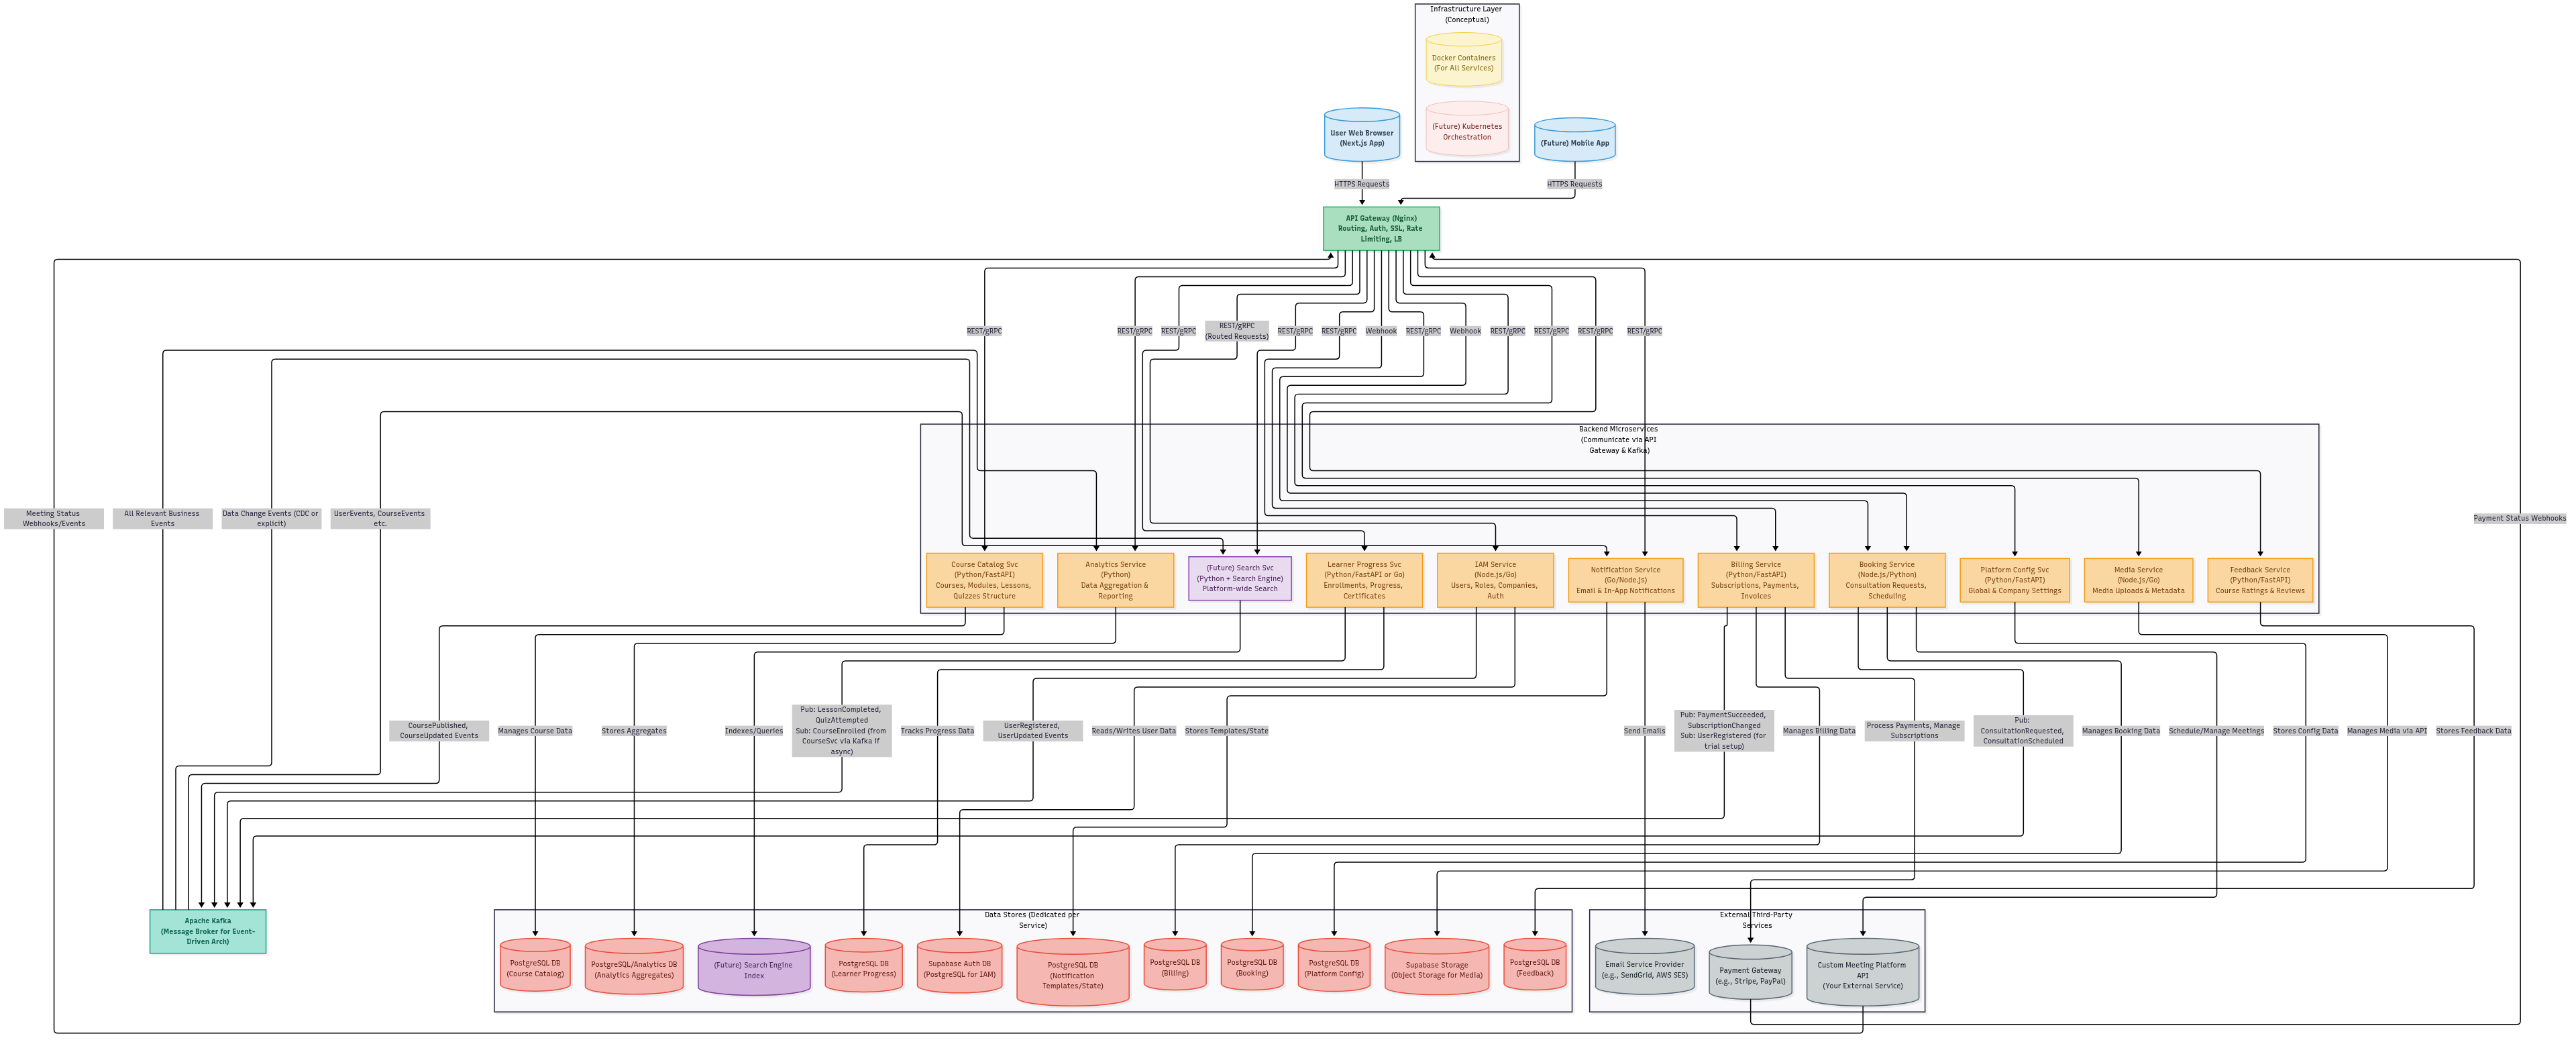
\includegraphics[width=0.9\textwidth,keepaspectratio]{archetecture_diagrame.png}
  \caption{\textbf{Diagramme d'architecture backend} et base de données de la plateforme e-learning.}
  \label{fig:architecture_diagram}
\end{figure}

Le diagramme ci-dessus illustre l'architecture microservices proposée, avec les différents services et leurs interactions. Cette architecture permettra un développement modulaire, une maintenance facilitée et une évolution progressive de la plateforme.

\subsection{Communication Inter-Services}
Pour illustrer le fonctionnement de l'architecture, voici un exemple de flux de communication entre les services pour un scénario d'inscription et d'abonnement :
\begin{enumerate}
  \item \textbf{Client (Next.js)} $\rightarrow$ \textbf{Passerelle API (Nginx)} $\rightarrow$ \textbf{Service IAM} (Création de l'utilisateur)
  \item \textbf{Service IAM} $\rightarrow$ \textbf{Kafka} (Publie `UserRegisteredEvent`)
  \item \textbf{Service de Notification} (Consomme l'événement) $\rightarrow$ Envoie un Email de Bienvenue
  \item \textbf{Client} $\rightarrow$ \textbf{Passerelle API} $\rightarrow$ \textbf{Service de Facturation} (Demande d'abonnement)
  \item \textbf{Service de Facturation} $\rightarrow$ Passerelle de Paiement et Mise à jour de la BD interne
  \item \textbf{Service de Facturation} $\rightarrow$ \textbf{Kafka} (Publie `SubscriptionActivatedEvent`)
  \item \textbf{Service IAM} (Consomme, met à jour le statut utilisateur) \& \textbf{Service de Notification} (Consomme, envoie une confirmation)
\end{enumerate}

Cette approche combine des appels API synchrones lorsque nécessaire et des flux événementiels asynchrones pour une meilleure résilience et scalabilité.

\subsection{Modèles de Données des Services}
Dans le cadre de cette première semaine, des modèles de données préliminaires ont été conçus pour chacun des services identifiés. Voici quelques exemples des structures de données principales :

\newpage
\subsubsection{Service IAM (Identity and Access Management)}
\begin{figure}[h!]
  \centering
  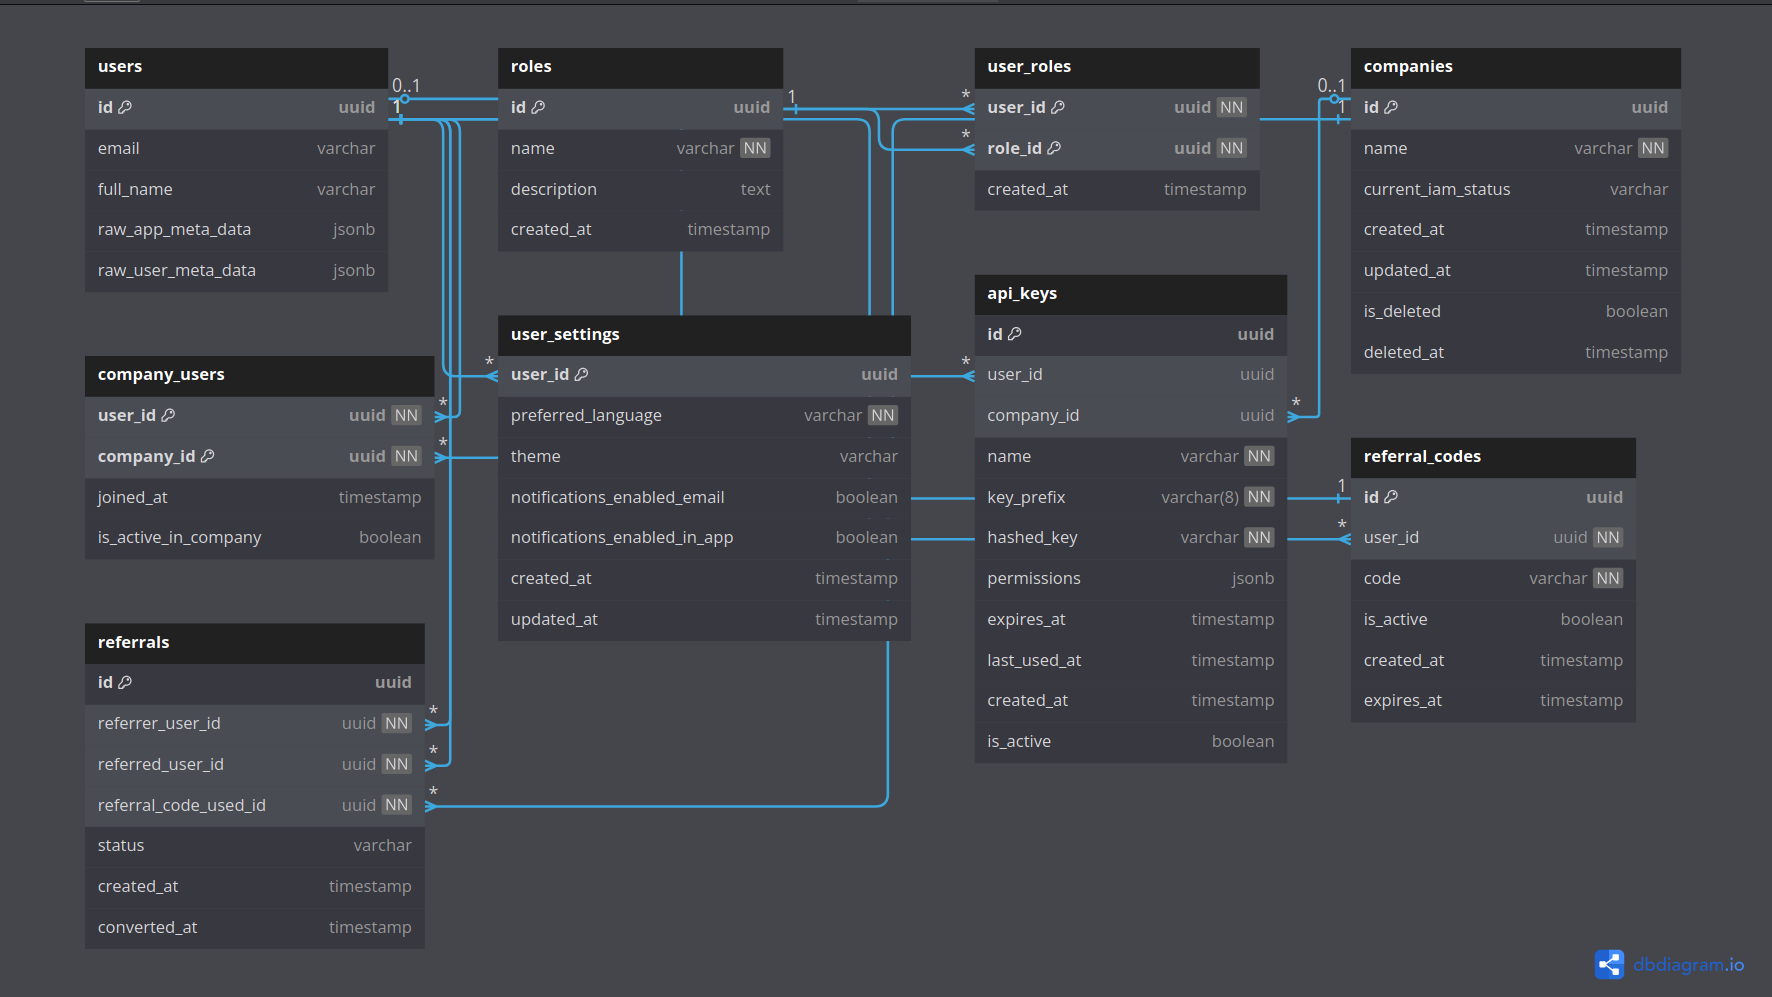
\includegraphics[width=0.8\textwidth,keepaspectratio]{services_db_screanshots/Screenshot 2025-06-06 at 15-08-36 IAM_Service.pdf.png}
  \caption{\textbf{Modèle de données du service IAM} pour la gestion des utilisateurs et des accès.}
  \label{fig:iam_service}
\end{figure}
\vspace{-10pt}
\small
\paragraph{Points clés du modèle IAM :}
\begin{itemize}[leftmargin=*,noitemsep,topsep=0pt]
  \item \textbf{Gestion centralisée des utilisateurs} avec tables dédiées aux utilisateurs, rôles et permissions
  \item \textbf{Support multi-tenant} via la table des entreprises (companies)
  \item \textbf{Système de référence} permettant le suivi des recommandations et affiliations
  \item \textbf{Paramètres utilisateurs} stockés de manière structurée pour personnaliser l'expérience
  \item \textbf{Jetons d'authentification} permettant une gestion sécurisée des sessions
\end{itemize}
\normalsize
\newpage

\subsubsection{Service de Contenu}
\begin{figure}[h!]
  \centering
  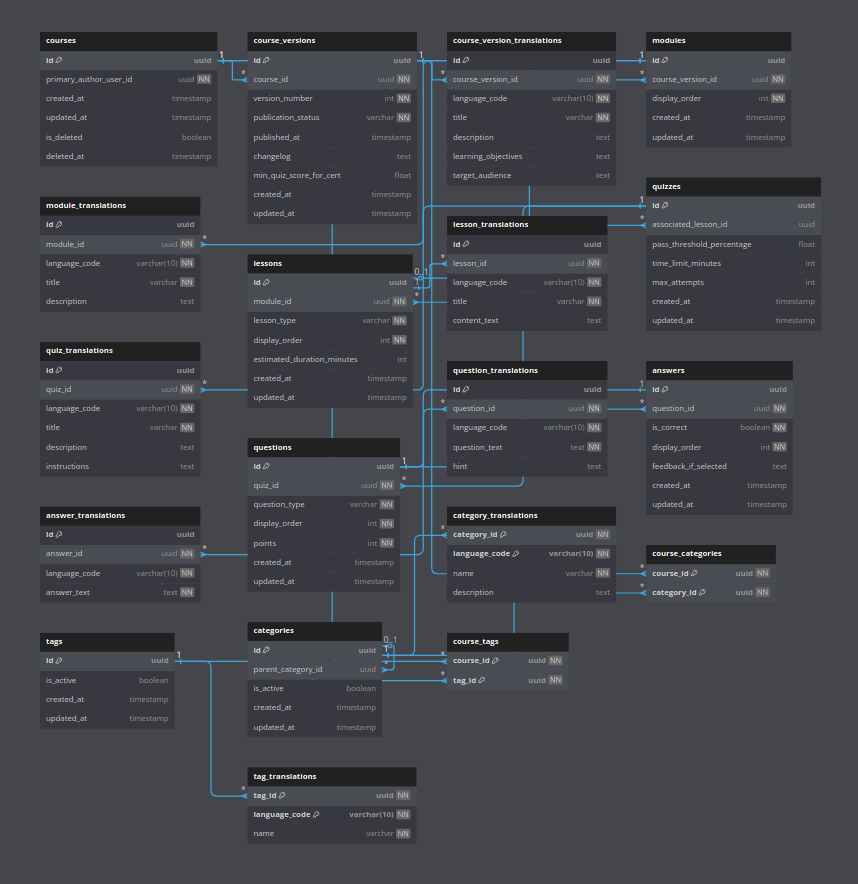
\includegraphics[width=0.8\textwidth,keepaspectratio]{services_db_screanshots/Screenshot 2025-06-06 at 15-07-51 Content_Service.pdf.png}
  \caption{\textbf{Modèle de données du service de contenu} pour la gestion des cours et du matériel pédagogique.}
  \label{fig:content_service}
\end{figure}
\vspace{-10pt}
\small
\paragraph{Points clés du service de Contenu :}
\begin{itemize}[leftmargin=*,noitemsep,topsep=0pt]
  \item \textbf{Structure hiérarchique} des cours, modules et leçons
  \item \textbf{Support multimédia} avec gestion des vidéos, documents et quizz
  \item \textbf{Métadonnées riches} pour faciliter la recherche et la catégorisation
  \item \textbf{Gestion des versions} permettant la mise à jour du contenu sans perte d'historique
  \item \textbf{Support multilingue} pour internationaliser le contenu pédagogique
\end{itemize}
\normalsize
\newpage

\subsubsection{Service de Facturation et d'Abonnement}
\begin{figure}[h!]
  \centering
  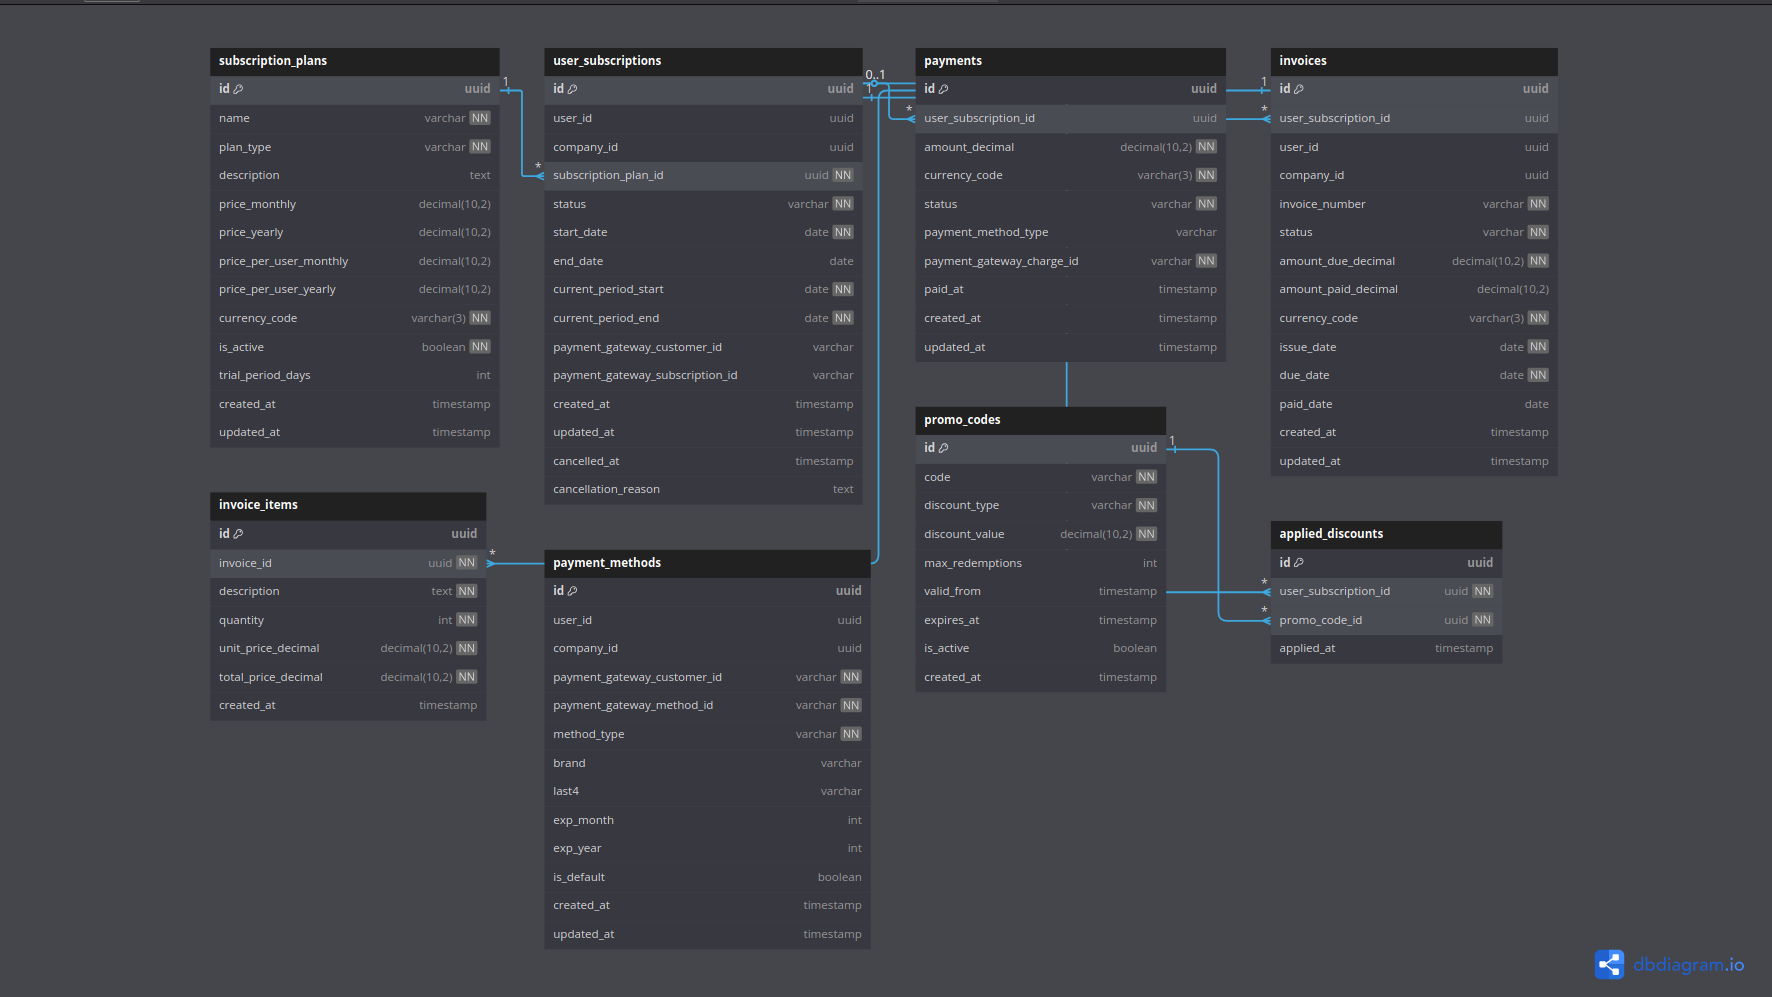
\includegraphics[width=0.8\textwidth,keepaspectratio]{services_db_screanshots/Screenshot 2025-06-06 at 15-05-28 Billing_and_Subscription_Service.pdf.png}
  \caption{\textbf{Modèle de données du service de facturation} pour la gestion des abonnements et des paiements.}
  \label{fig:billing_service}
\end{figure}
\vspace{-10pt}
\small
\paragraph{Points clés du service de Facturation :}
\begin{itemize}[leftmargin=*,noitemsep,topsep=0pt]
  \item \textbf{Gestion des plans d'abonnement} avec différents niveaux de service
  \item \textbf{Suivi des factures et paiements} pour les utilisateurs individuels et entreprises
  \item \textbf{Support des promotions et réductions} temporaires ou permanentes
  \item \textbf{Historique de facturation} complet pour analyses financières
  \item \textbf{Intégration} avec les passerelles de paiement externes
\end{itemize}
\normalsize
\newpage

\subsubsection{Service de Certification}
\begin{figure}[h!]
  \centering
  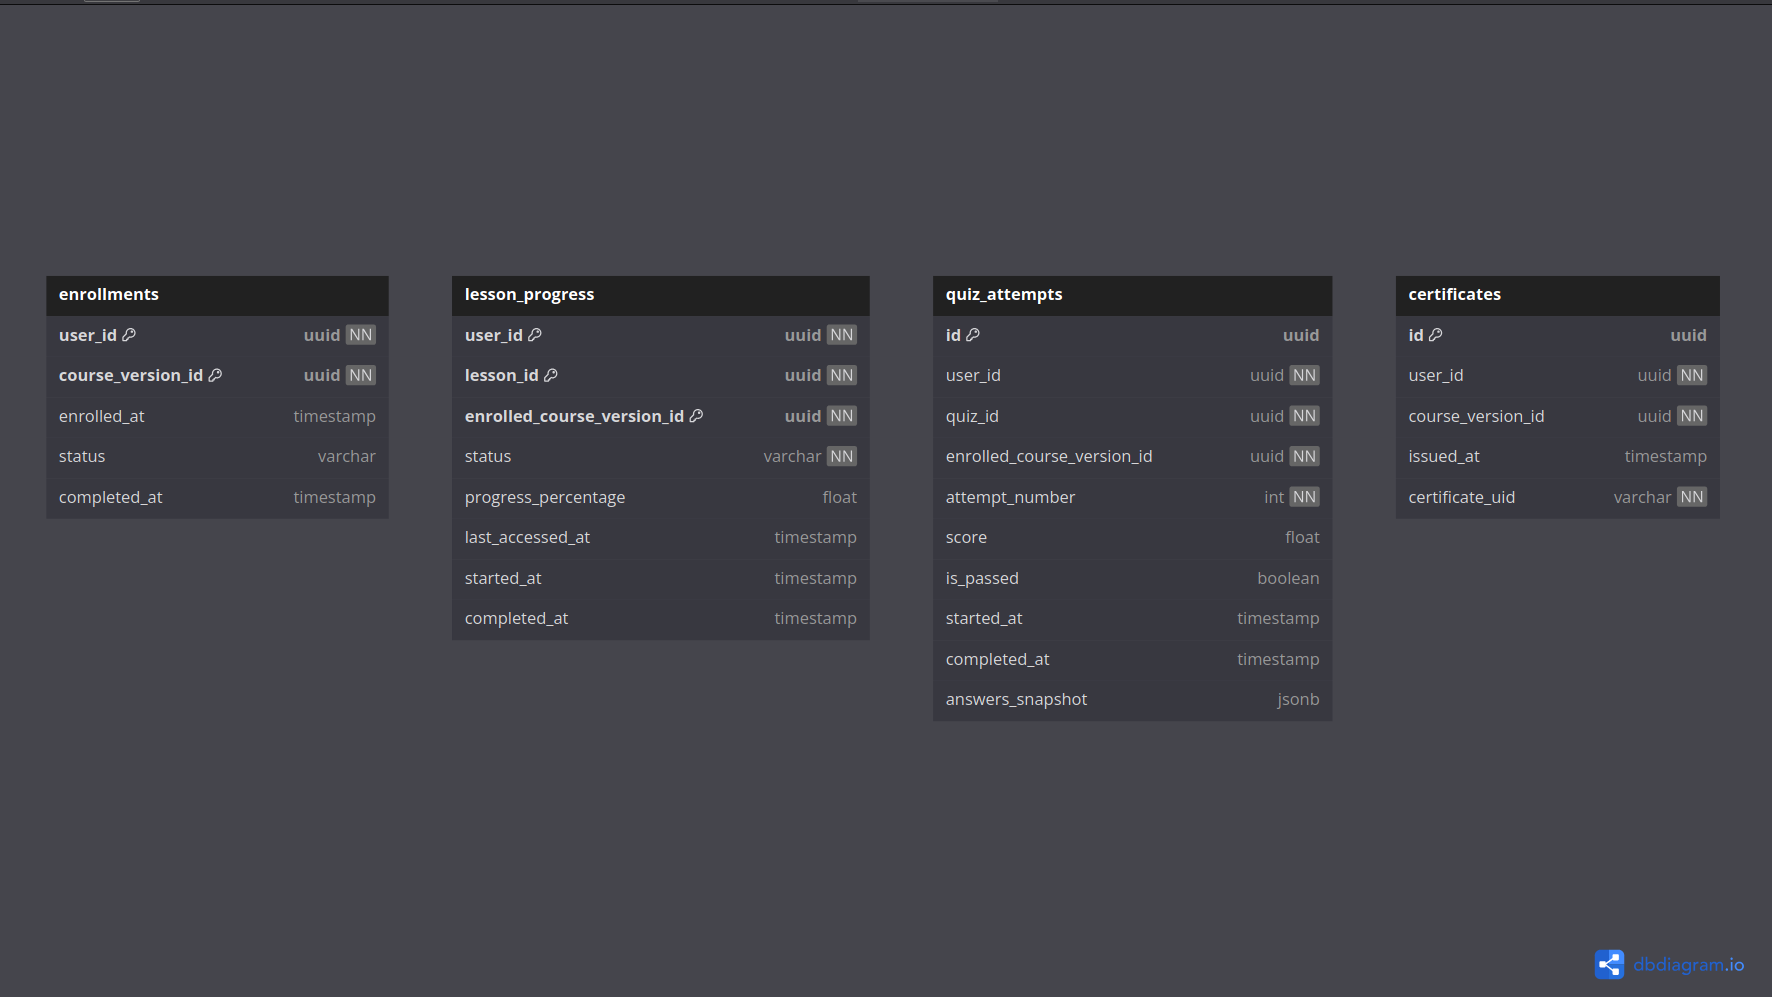
\includegraphics[width=0.8\textwidth,keepaspectratio]{services_db_screanshots/Screenshot 2025-06-06 at 15-05-53 Certification_Service.pdf.png}
  \caption{\textbf{Modèle de données du service de certification} pour la délivrance et la validation des certificats.}
  \label{fig:certification_service}
\end{figure}
\vspace{-10pt}
\small
\paragraph{Points clés du service de Certification :}
\begin{itemize}[leftmargin=*,noitemsep,topsep=0pt]
  \item \textbf{Création de certificats} à l'achèvement des cours et modules
  \item \textbf{Validation et vérification} des compétences acquises
  \item \textbf{Badges et récompenses} pour motiver les apprenants
  \item \textbf{Système de validation externe} permettant aux entreprises de vérifier l'authenticité
  \item \textbf{Historique des certifications} pour chaque utilisateur
\end{itemize}
\normalsize
\newpage

\subsubsection{Service d'Analytique et Reporting}
\begin{figure}[h!]
  \centering
  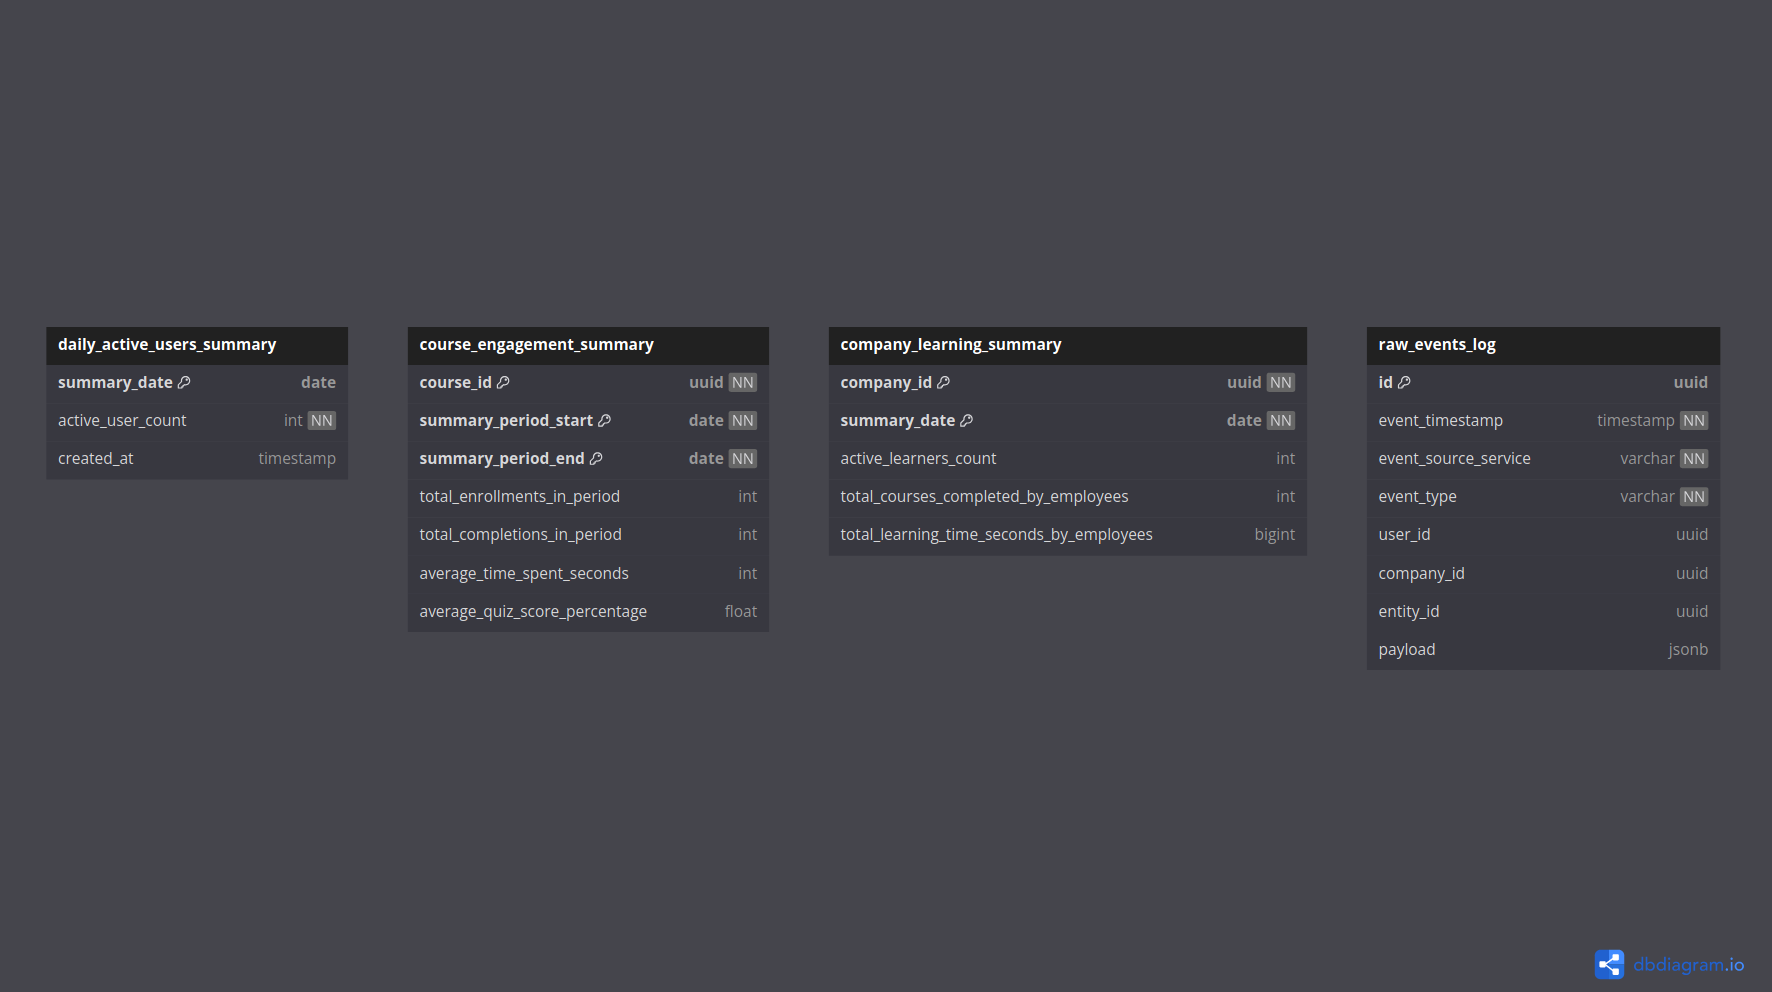
\includegraphics[width=0.8\textwidth,keepaspectratio]{services_db_screanshots/Screenshot 2025-06-06 at 15-04-59 Analytics_and_Reporting_Service.pdf.png}
  \caption{\textbf{Modèle de données du service d'analytique} pour le suivi des performances et la génération de rapports.}
  \label{fig:analytics_service}
\end{figure}
\vspace{-10pt}
\small
\paragraph{Points clés du service d'Analytique :}
\begin{itemize}[leftmargin=*,noitemsep,topsep=0pt]
  \item \textbf{Collecte de données d'utilisation} sur toutes les interactions utilisateurs
  \item \textbf{Métriques de performance} pour les cours et modules
  \item \textbf{Rapports personnalisés} pour les administrateurs et entreprises
  \item \textbf{Tableaux de bord en temps réel} pour le suivi des indicateurs clés
  \item \textbf{Système d'alerte} pour identifier les anomalies ou opportunités
\end{itemize}
\normalsize
\newpage

\subsubsection{Service de Feedback}
\begin{figure}[h!]
  \centering
  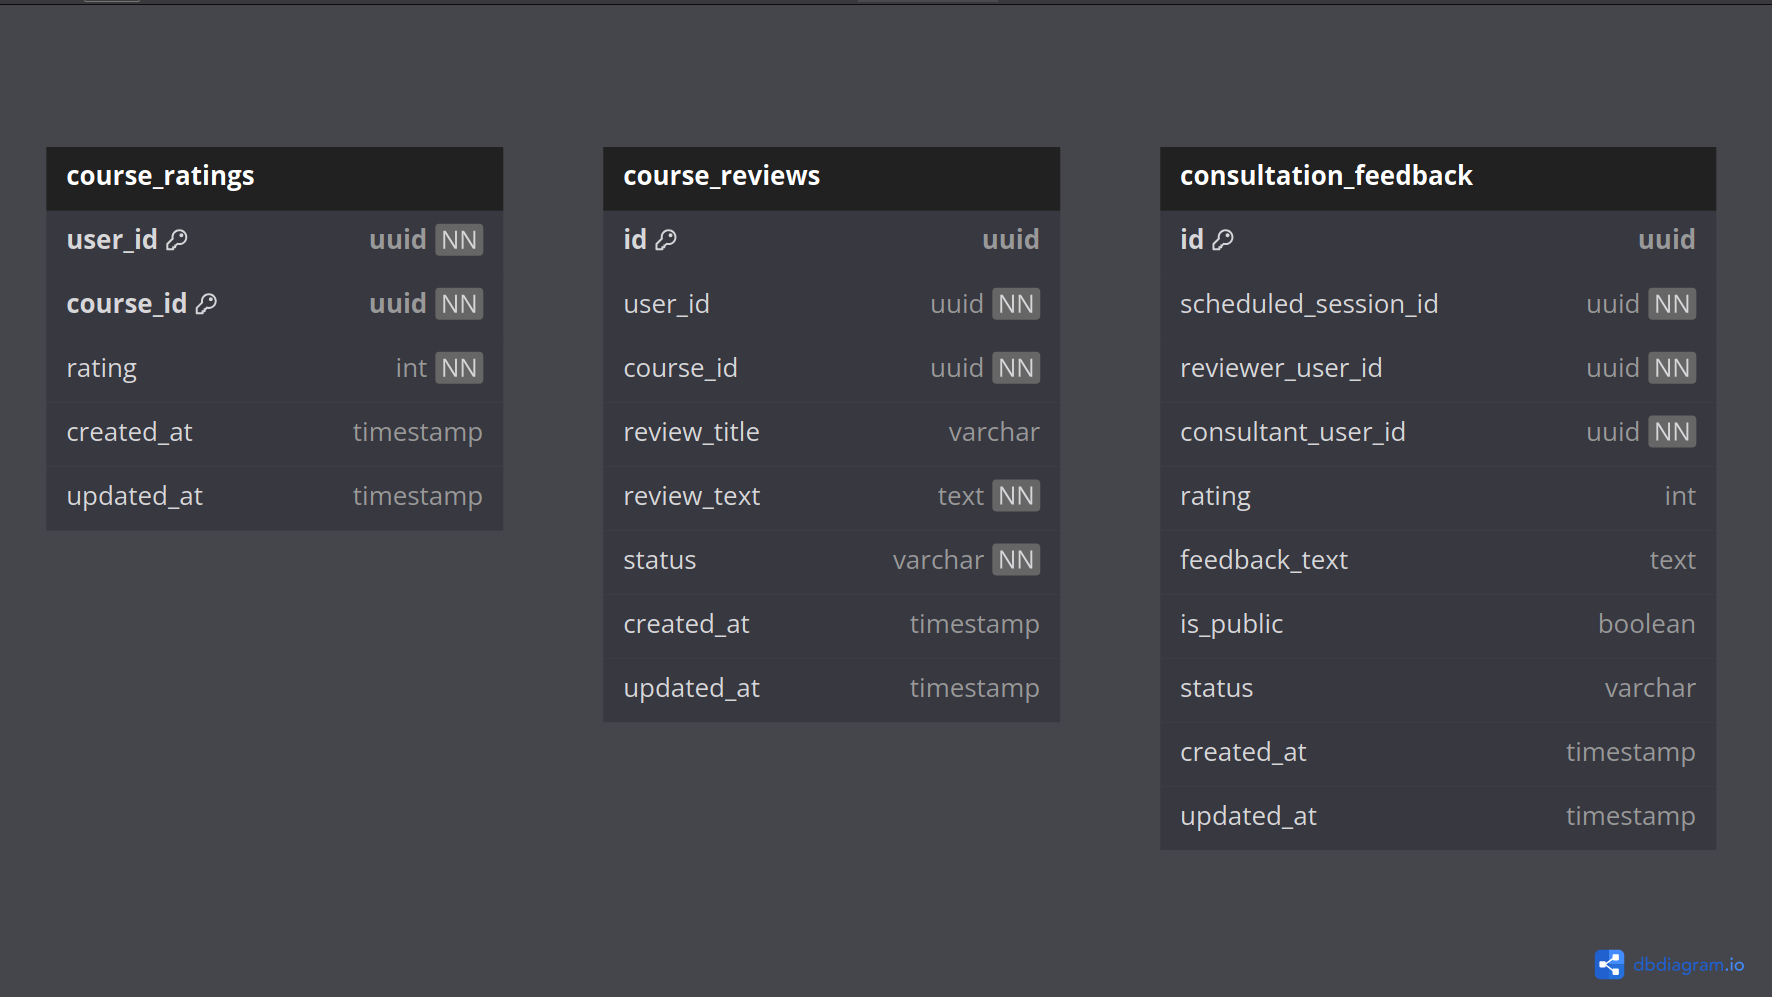
\includegraphics[width=0.8\textwidth,keepaspectratio]{services_db_screanshots/Screenshot 2025-06-06 at 15-08-00 Feedback_Service.pdf.png}
  \caption{\textbf{Modèle de données du service de feedback} pour la collecte et la gestion des retours utilisateurs.}
  \label{fig:feedback_service}
\end{figure}
\vspace{-10pt}
\small
\paragraph{Points clés du service de Feedback :}
\begin{itemize}[leftmargin=*,noitemsep,topsep=0pt]
  \item \textbf{Évaluations et avis} sur les cours et modules
  \item \textbf{Système de notation} permettant une évaluation quantitative
  \item \textbf{Commentaires et suggestions} pour améliorer le contenu
  \item \textbf{Analyse de sentiment} sur les retours textuels
  \item \textbf{Boucle de rétroaction} pour les créateurs de contenu
\end{itemize}
\normalsize
\newpage

\subsubsection{Service de Notification}
\begin{figure}[h!]
  \centering
  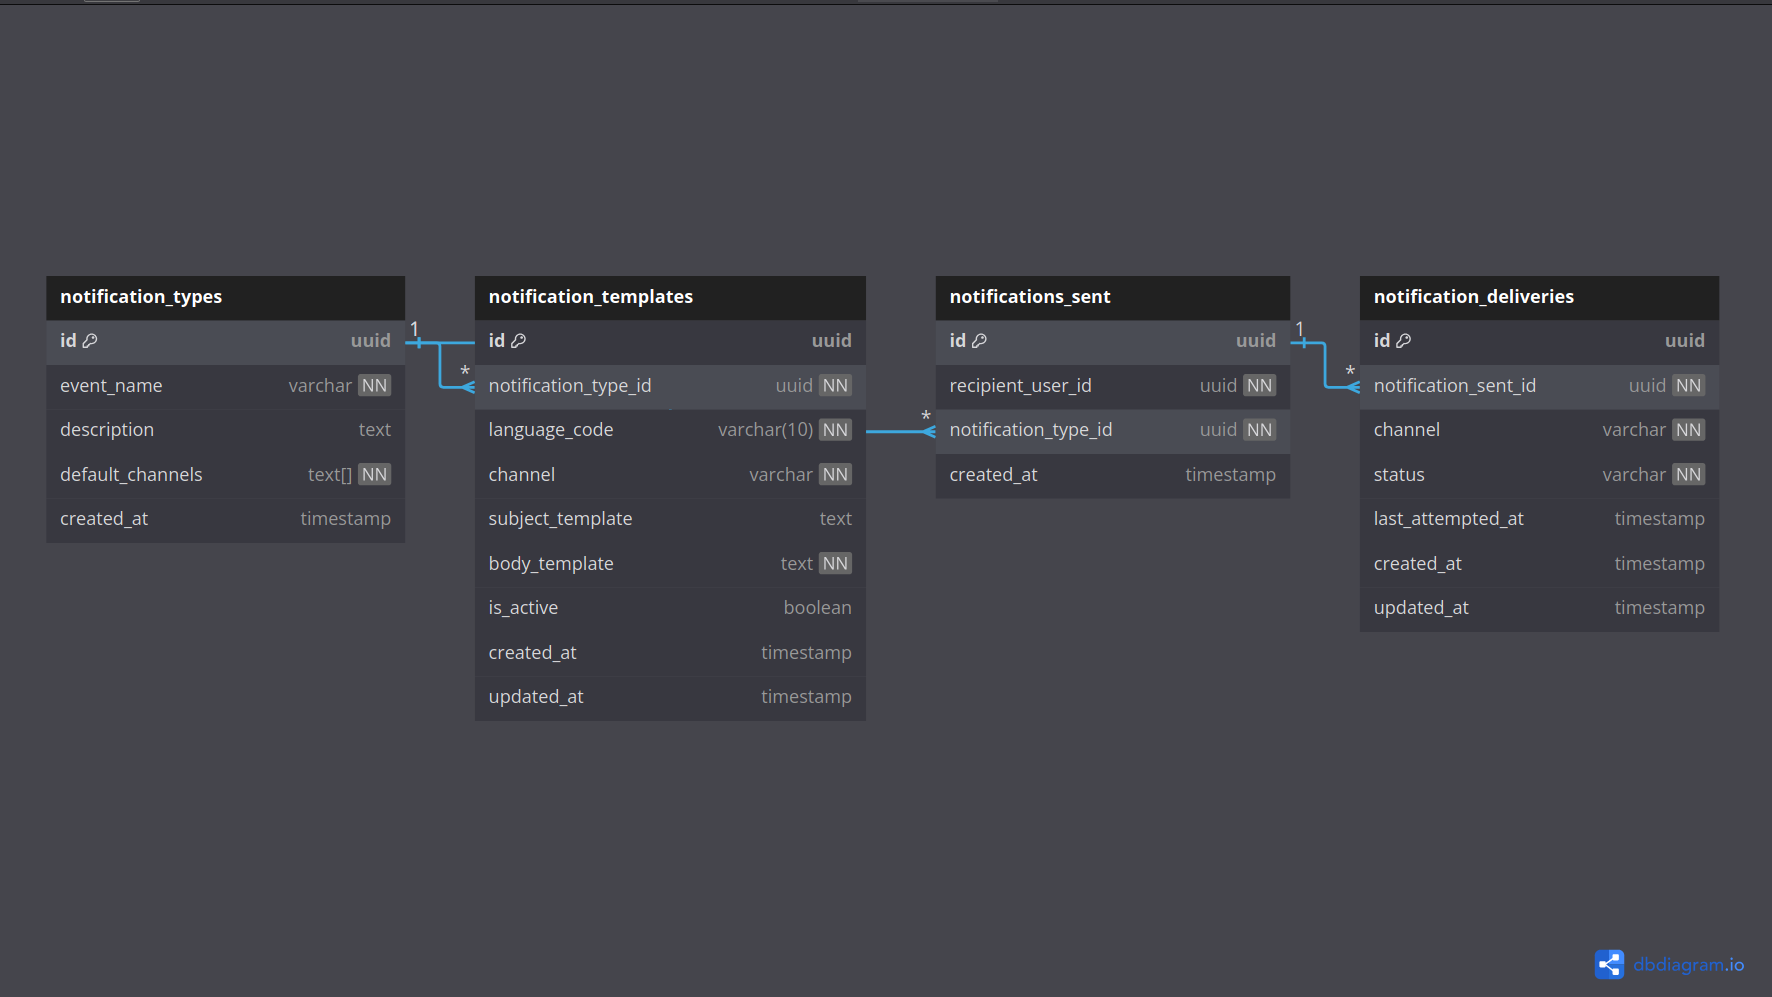
\includegraphics[width=0.8\textwidth,keepaspectratio]{services_db_screanshots/Screenshot 2025-06-06 at 15-08-13 Notification_Service.pdf.png}
  \caption{\textbf{Modèle de données du service de notification} pour l'envoi et la gestion des notifications.}
  \label{fig:notification_service}
\end{figure}
\vspace{-10pt}
\small
\paragraph{Points clés du service de Notification :}
\begin{itemize}[leftmargin=*,noitemsep,topsep=0pt]
  \item \textbf{Notifications temps réel} pour les événements importants
  \item \textbf{Préférences de notification} configurables par utilisateur
  \item \textbf{Support multi-canal} : email, push, in-app, SMS
  \item \textbf{Modèles de messages} personnalisables
  \item \textbf{Planification et automatisation} des campagnes de notification
\end{itemize}
\normalsize
\newpage

\subsubsection{Service de Gestion des Médias}
\begin{figure}[h!]
  \centering
  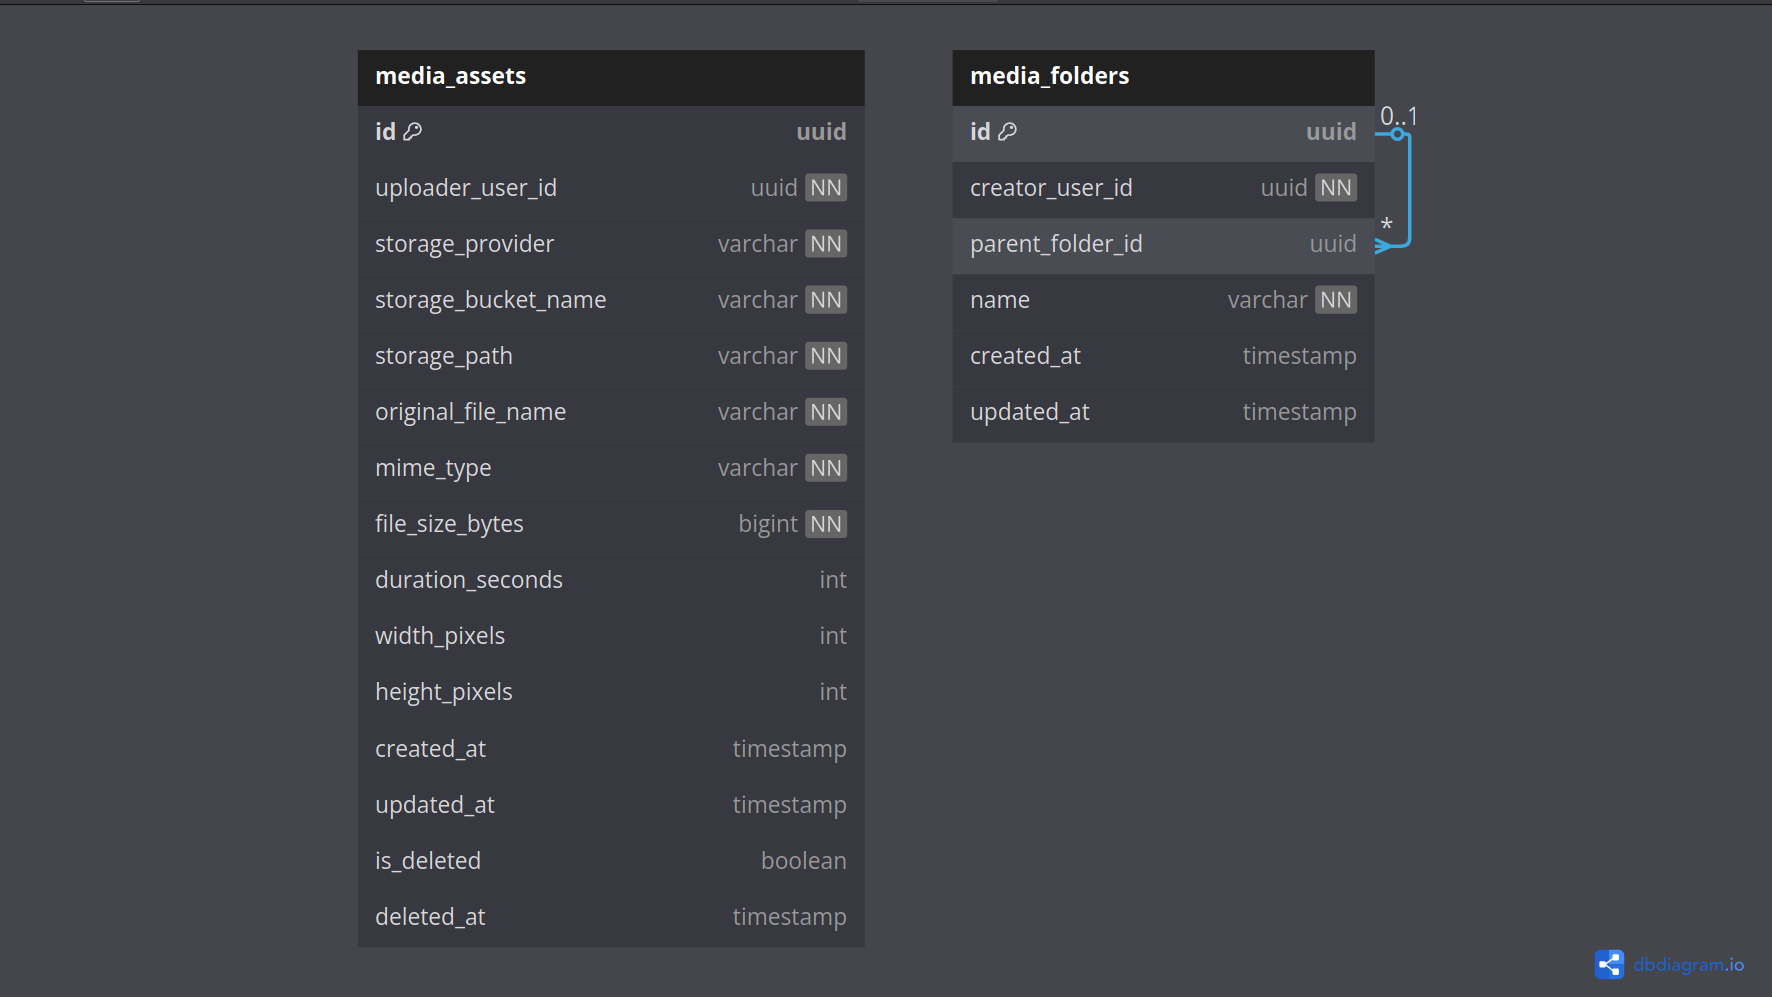
\includegraphics[width=0.8\textwidth,keepaspectratio]{services_db_screanshots/Screenshot 2025-06-06 at 15-08-27 Media_Management_Service.pdf.png}
  \caption{\textbf{Modèle de données du service de gestion des médias} pour le stockage et l'accès aux ressources multimédias.}
  \label{fig:media_service}
\end{figure}
\vspace{-10pt}
\small
\paragraph{Points clés du service de Médias :}
\begin{itemize}[leftmargin=*,noitemsep,topsep=0pt]
  \item \textbf{Gestion centralisée} des ressources audio, vidéo et images
  \item \textbf{Métadonnées enrichies} pour faciliter la recherche et l'organisation
  \item \textbf{Support de multiples formats} et résolutions
  \item \textbf{Optimisation automatique} pour différents appareils
  \item \textbf{Contrôle des droits d'accès} pour les ressources protégées
\end{itemize}
\normalsize
\newpage

\subsubsection{Service de Configuration de la Plateforme}
\begin{figure}[h!]
  \centering
  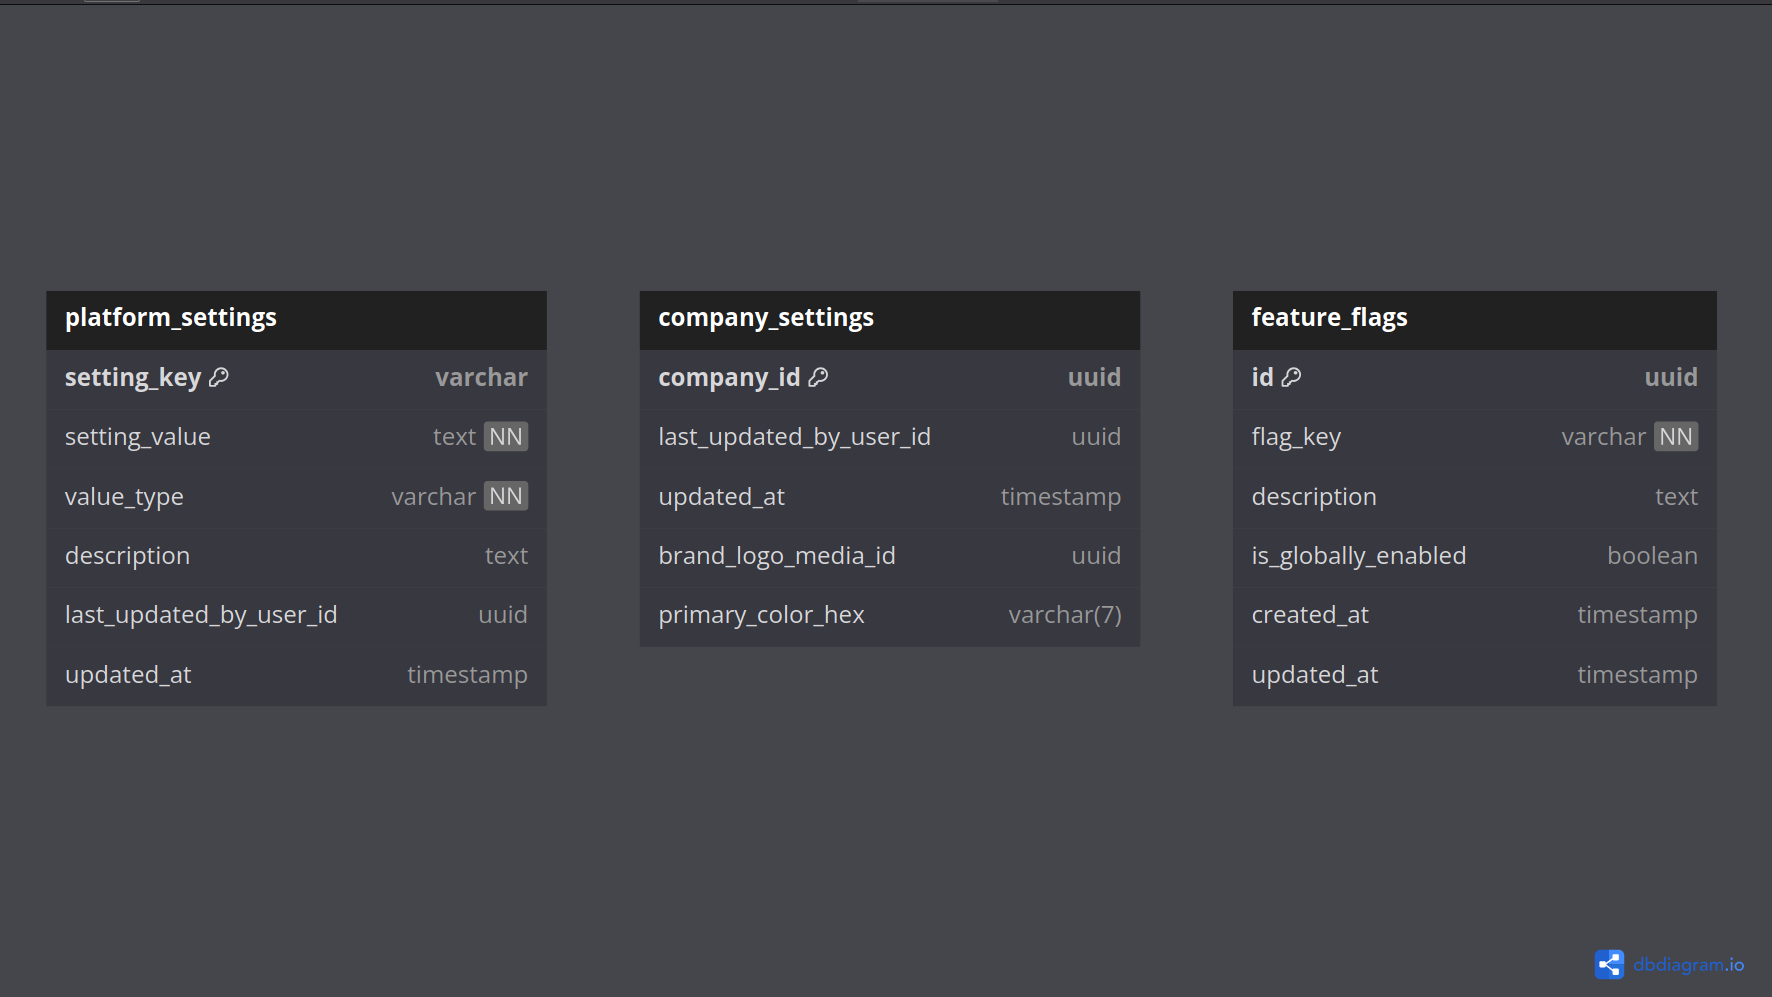
\includegraphics[width=0.8\textwidth,keepaspectratio]{services_db_screanshots/Screenshot 2025-06-06 at 15-08-44 Platform_Configuration_Service.pdf.png}
  \caption{\textbf{Modèle de données du service de configuration} pour la gestion des paramètres globaux de la plateforme.}
  \label{fig:platform_config_service}
\end{figure}
\vspace{-10pt}
\small
\paragraph{Points clés du service de Configuration :}
\begin{itemize}[leftmargin=*,noitemsep,topsep=0pt]
  \item \textbf{Paramètres système} centralisés et accessibles à tous les services
  \item \textbf{Gestion des drapeaux de fonctionnalités} (feature flags)
  \item \textbf{Configuration par environnement} (développement, test, production)
  \item \textbf{Personnalisation de l'interface} selon les besoins spécifiques
  \item \textbf{Paramètres multilingues} pour localisation de la plateforme
\end{itemize}
\normalsize
\newpage

\subsubsection{Service de Recherche}
\begin{figure}[h!]
  \centering
  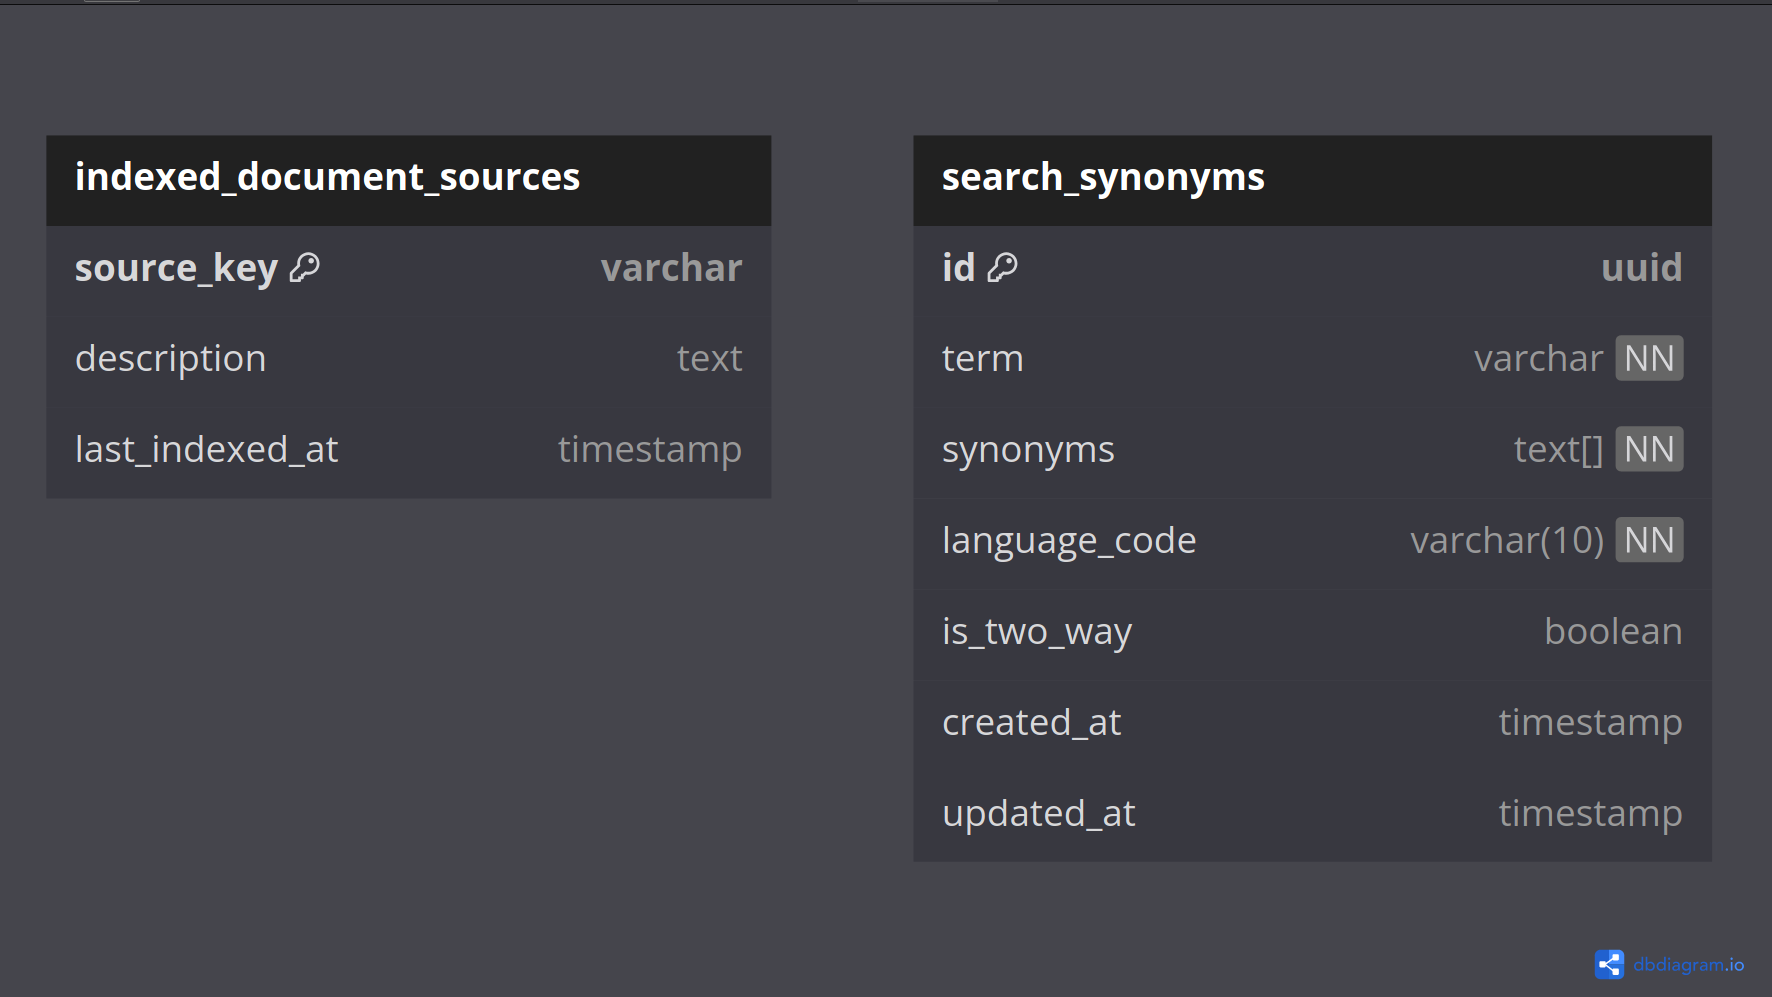
\includegraphics[width=0.8\textwidth,keepaspectratio]{services_db_screanshots/Screenshot 2025-06-06 at 15-08-52 Search_Service.pdf.png}
  \caption{\textbf{Modèle de données du service de recherche} pour l'indexation et la recherche de contenu.}
  \label{fig:search_service}
\end{figure}
\vspace{-10pt}
\small
\paragraph{Points clés du service de Recherche :}
\begin{itemize}[leftmargin=*,noitemsep,topsep=0pt]
  \item \textbf{Indexation intelligente} du contenu des cours et ressources
  \item \textbf{Recherche full-text} avec prise en charge des synonymes
  \item \textbf{Système de tags} pour améliorer la pertinence des résultats
  \item \textbf{Historique des recherches} pour l'analyse des tendances
  \item \textbf{Algorithme de recommandation} basé sur les comportements de recherche
\end{itemize}

\begin{table}[h!]
\centering
\small
\caption{Comparaison des caractéristiques techniques des services}
\label{tab:comparaison_services}
\begin{tabular}{|l|c|c|c|}
\hline
\textbf{Service} & \textbf{Technologie principale} & \textbf{Type de données} & \textbf{Complexité} \\
\hline
IAM & Node.js/Go & Utilisateurs & Élevée \\
Contenu & Python/FastAPI & Éducation & Moyenne \\
Facturation & Python/FastAPI & Financières & Élevée \\
Certification & Python/Go & Validation & Moyenne \\
Analytique & Python & Statistiques & Élevée \\
Feedback & Node.js & Évaluation & Basse \\
Notification & Go & Messaging & Moyenne \\
Médias & Node.js & Binaires & Élevée \\
Configuration & Go & Paramètres & Basse \\
Recherche & Python/Elasticsearch & Index & Élevée \\
\hline
\end{tabular}
\end{table}
\normalsize 

% Week 2 content
\chapter{Semaine 2 : Conception de l'Interface d'Accueil}
\thispagestyle{fancy}

La deuxième semaine du stage a été consacrée au développement de l'interface d'accueil de la plateforme e-learning. Cette étape était cruciale pour établir l'identité visuelle du projet et créer une première impression positive auprès des utilisateurs.

\section{Conception de la Page d'Accueil}

La page d'accueil a été conçue pour présenter clairement la valeur ajoutée de la plateforme et inciter les utilisateurs à s'inscrire. Plusieurs sections ont été développées pour structurer l'information de manière efficace.

\subsection{Hero Section}
La section principale (Hero Section) a été conçue pour capturer immédiatement l'attention des visiteurs avec un message clair et une incitation à l'action.

\begin{figure}[h!]
  \centering
  
\includegraphics[width=0.9\textwidth,keepaspectratio]{week_2_img/last_and_improved_hero_section_withe_3d_effects_etc.png}
  \caption{\textbf{Hero Section améliorée} de la page d'accueil avec effets 3D et animations interactives.}
  \label{fig:hero_section_improved}
\end{figure}

Les éléments clés de cette section comprennent :
\begin{itemize}
  \item Un titre accrocheur qui met en avant la proposition de valeur principale
  \item Un sous-titre explicatif sur les avantages de la plateforme
  \item Un bouton d'appel à l'action bien visible pour l'inscription
  \item Une illustration moderne avec des effets 3D représentant le concept d'apprentissage en ligne
  \item Un design responsive qui s'adapte à tous les types d'écrans
  \item Des animations interactives qui s'activent au survol ou au défilement
\end{itemize}

\subsection{Section "Where We Are"}
Une section spécifique a été développée pour illustrer la portée géographique et l'influence de la plateforme, renforçant ainsi sa crédibilité auprès des utilisateurs potentiels.

\begin{figure}[h!]
  \centering
  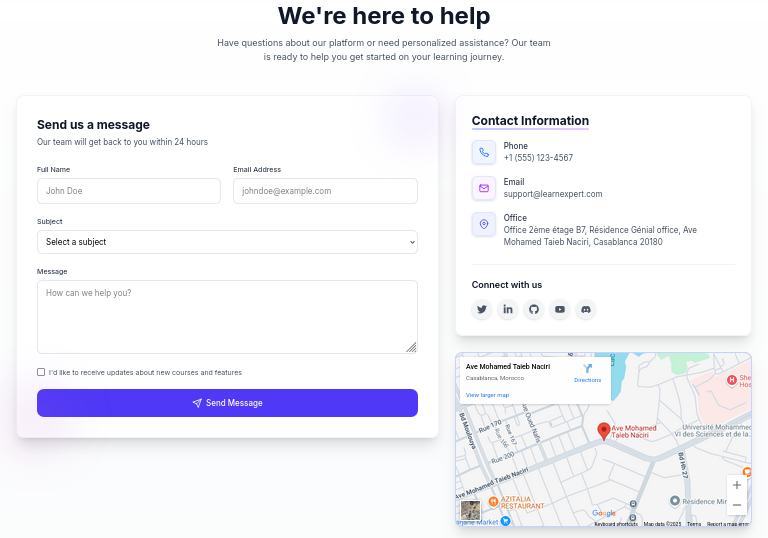
\includegraphics[width=0.9\textwidth,keepaspectratio]{week_2_img/where_we_are_section.png}
  \caption{\textbf{Section "Where We Are"} présentant la présence globale de la plateforme.}
  \label{fig:where_we_are}
\end{figure}

Cette section met en évidence :
\begin{itemize}
  \item Une carte interactive montrant la présence internationale
  \item Des statistiques sur le nombre d'utilisateurs par région
  \item Des témoignages d'utilisateurs de différentes zones géographiques
  \item Une visualisation de la croissance de la communauté mondiale
\end{itemize}

\subsection{Sections de Fonctionnalités}
Pour mettre en évidence les principales fonctionnalités de la plateforme, trois sections distinctes ont été développées, chacune mettant en avant un aspect spécifique de l'offre.

\begin{figure}[h!]
  \centering
  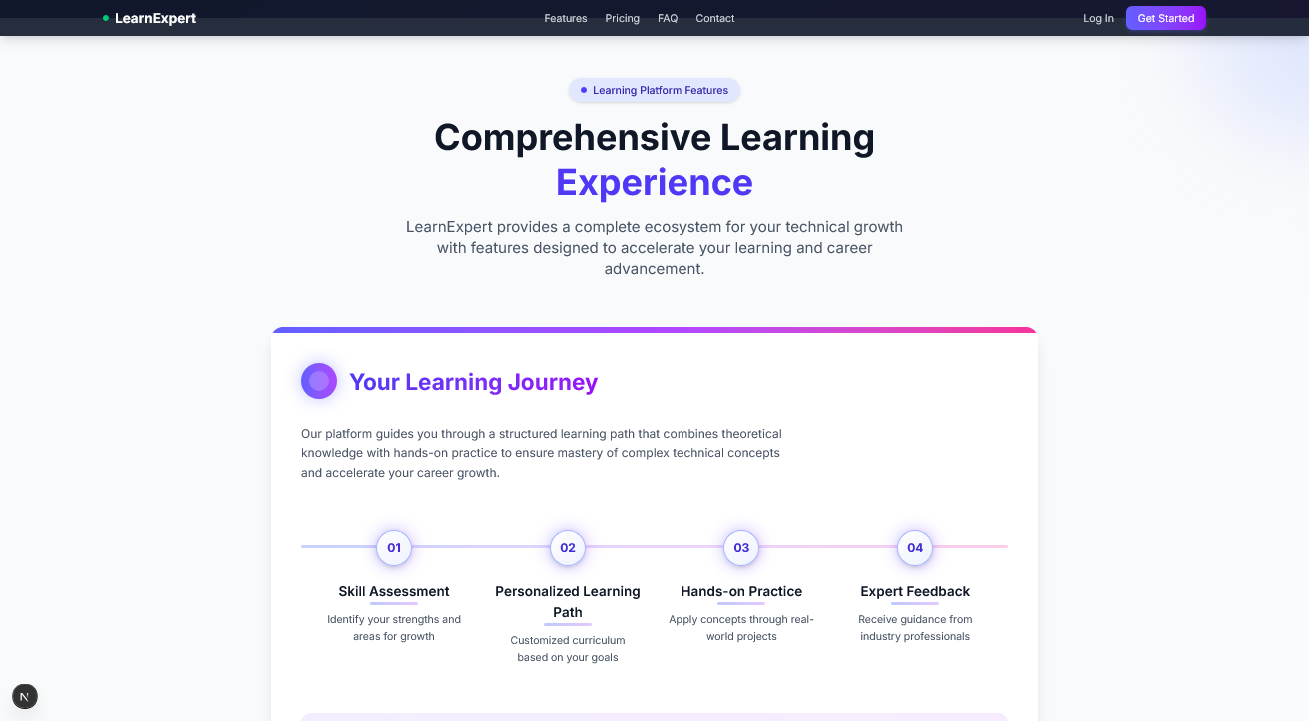
\includegraphics[width=0.9\textwidth,keepaspectratio]{week_2_img/featchersection_1.png}
  \caption{\textbf{Première section de fonctionnalités} présentant les cours en ligne.}
  \label{fig:features_section_1}
\end{figure}

\begin{figure}[h!]
  \centering
  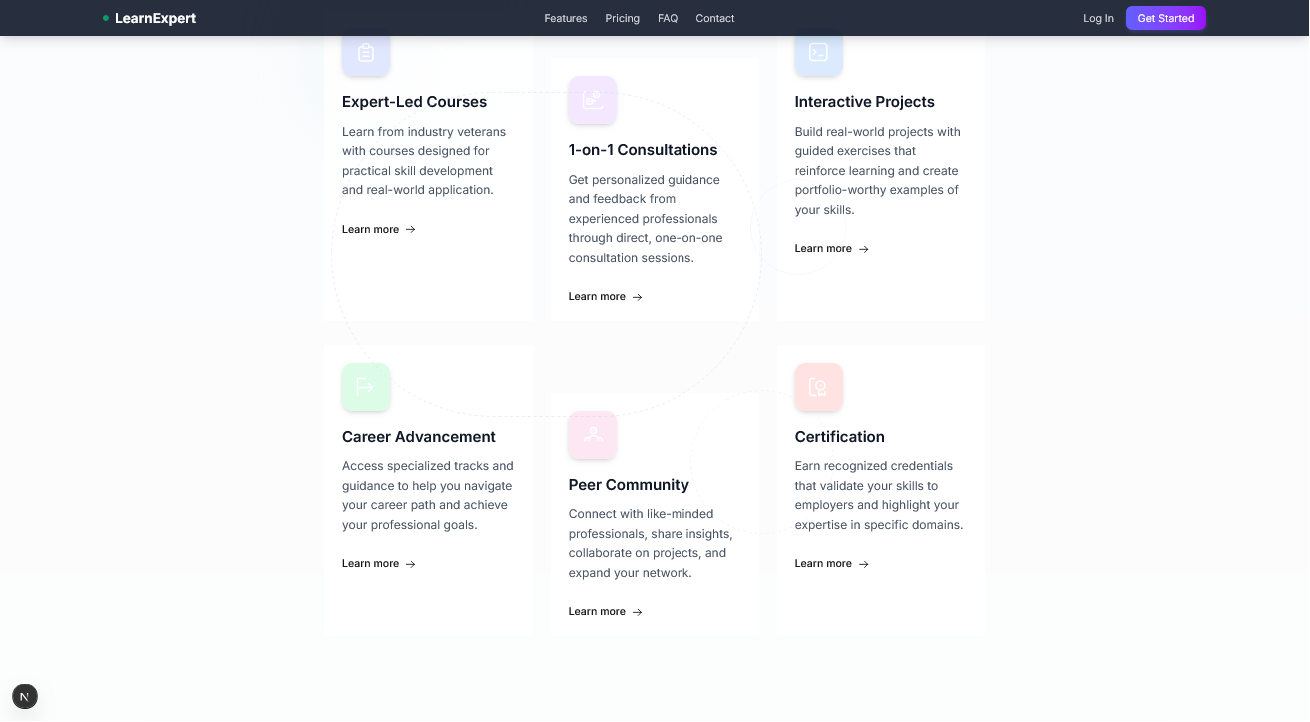
\includegraphics[width=0.9\textwidth,keepaspectratio]{week_2_img/fetchersection_2.png}
  \caption{\textbf{Deuxième section de fonctionnalités} mettant en avant les services de consultation.}
  \label{fig:features_section_2}
\end{figure}

\begin{figure}[h!]
  \centering
  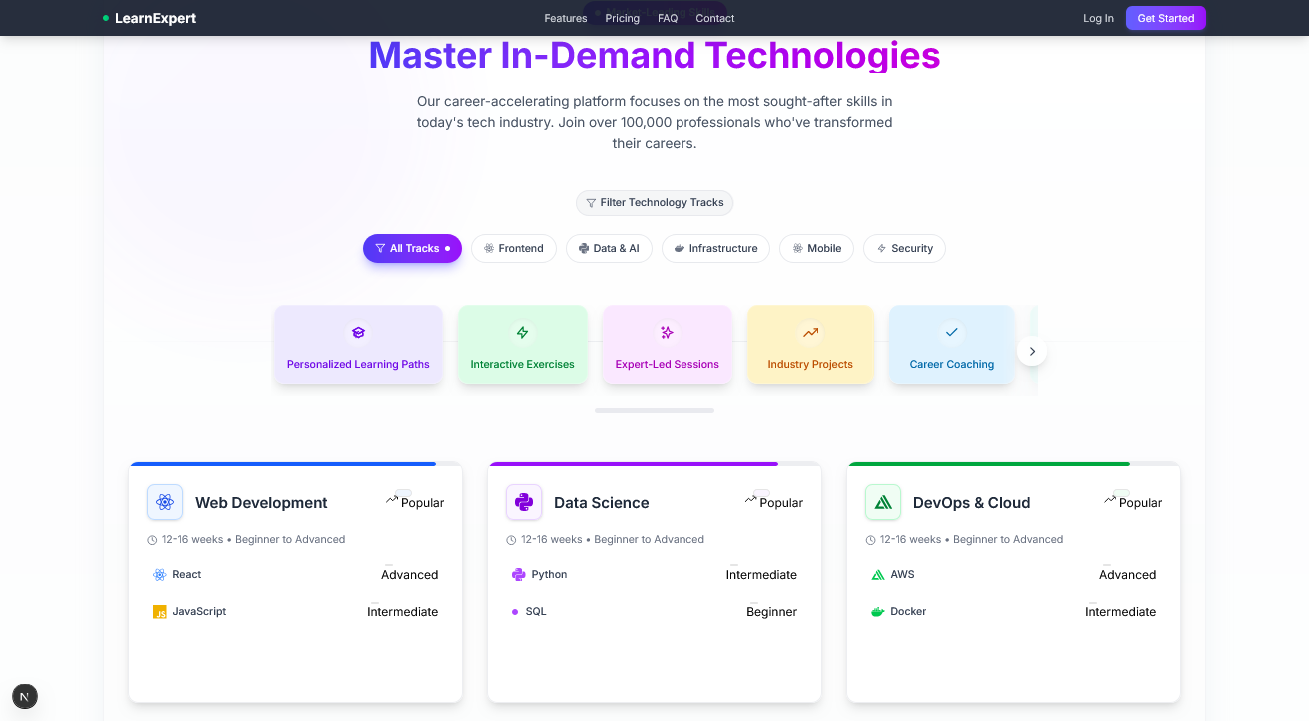
\includegraphics[width=0.9\textwidth,keepaspectratio]{week_2_img/fetchersection_3.png}
  \caption{\textbf{Troisième section de fonctionnalités} présentant les outils d'analyse et de suivi.}
  \label{fig:features_section_3}
\end{figure}

Chaque section de fonctionnalités comprend :
\begin{itemize}
  \item Une illustration ou icône représentative
  \item Un titre explicite de la fonctionnalité
  \item Une description détaillée des avantages
  \item Une mise en page alternée (image à gauche, texte à droite et inversement) pour créer un rythme visuel
\end{itemize}

\subsection{Section FAQ}
Pour répondre aux questions fréquentes des utilisateurs potentiels, une section FAQ interactive a été développée avec un système d'accordéon permettant de masquer/afficher les réponses.

\begin{figure}[h!]
  \centering
  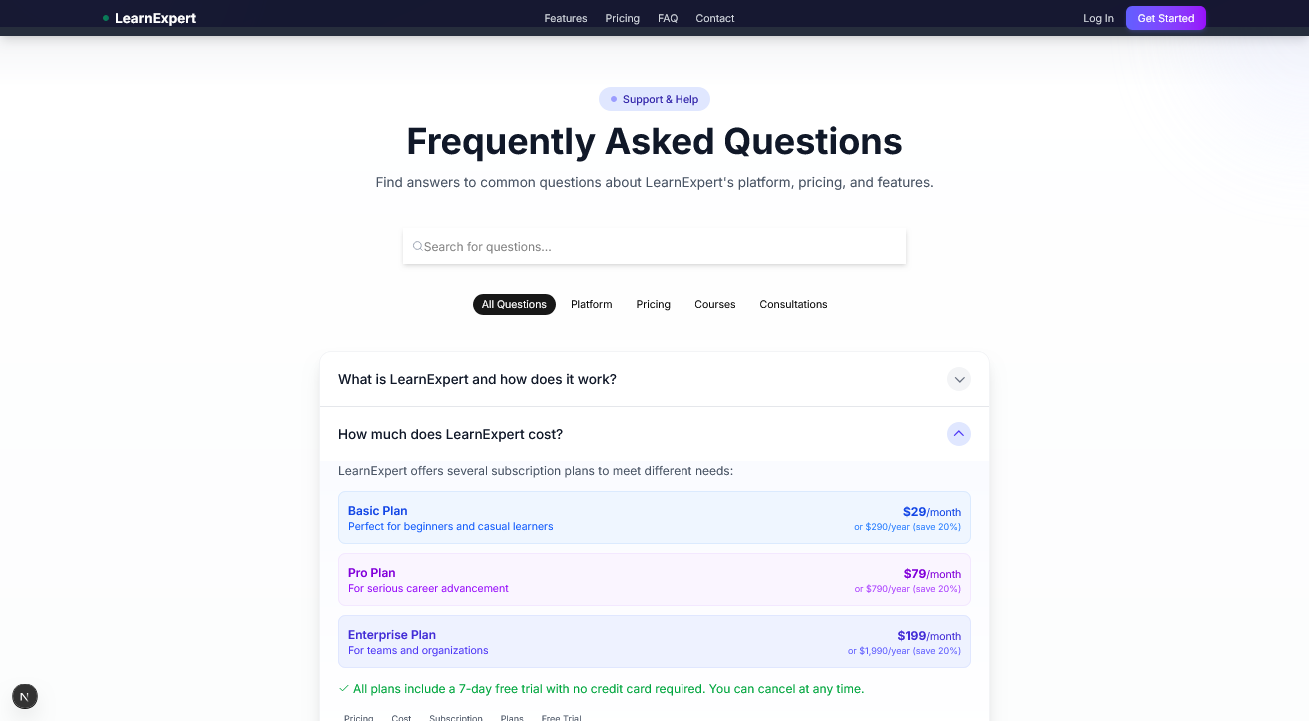
\includegraphics[width=0.9\textwidth,keepaspectratio]{week_2_img/faqsection.png}
  \caption{\textbf{Section FAQ} avec questions-réponses interactives.}
  \label{fig:faq_section}
\end{figure}

\subsection{Appel à l'Action Final}
Une seconde section d'appel à l'action a été ajoutée en bas de page pour inciter les utilisateurs ayant parcouru l'ensemble du contenu à s'inscrire.

\begin{figure}[h!]
  \centering
  
\includegraphics[width=0.9\textwidth,keepaspectratio]{week_2_img/second_call_of_action.png}
  \caption{\textbf{Section d'appel à l'action finale} incitant à l'inscription.}
  \label{fig:final_cta}
\end{figure}

\subsection{Barre de Navigation et Pied de Page}
La barre de navigation et le pied de page ont été conçus pour offrir un accès facile aux différentes sections du site et renforcer la crédibilité de la plateforme.

\begin{figure}[h!]
  \centering
  
\includegraphics[width=0.9\textwidth,keepaspectratio]{week_2_img/navbar.png}
  \caption{\textbf{Barre de navigation} avec les liens vers les principales sections.}
  \label{fig:navbar}
\end{figure}

\begin{figure}[h!]
  \centering
  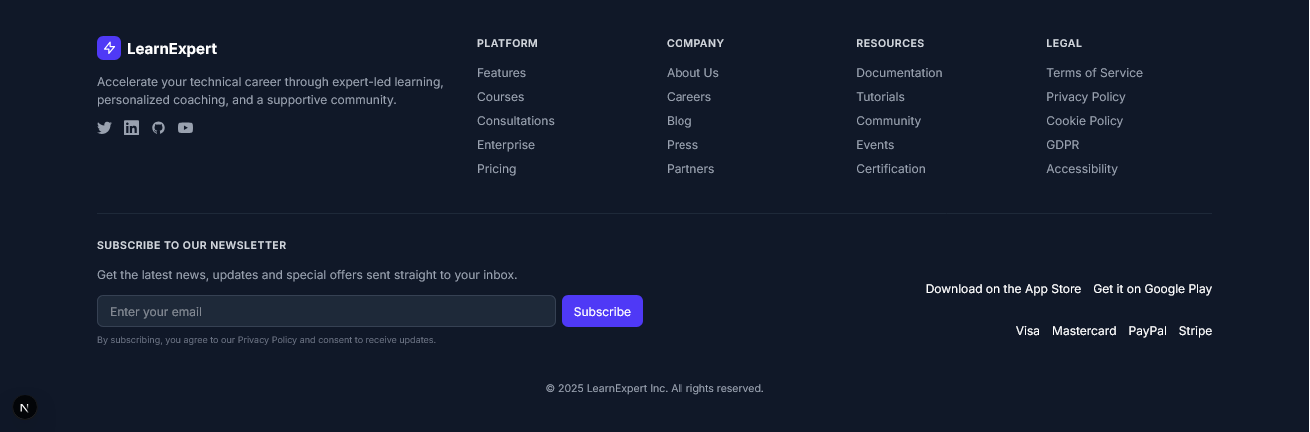
\includegraphics[width=0.9\textwidth,keepaspectratio]{week_2_img/foter.png}
  \caption{\textbf{Pied de page} avec informations légales et liens supplémentaires.}
  \label{fig:footer}
\end{figure}

\section{Mise en Place du Système de Paiement}

Un système de paiement sécurisé a également été intégré à la plateforme pour permettre l'achat d'abonnements et de services.

\begin{figure}[h!]
  \centering
  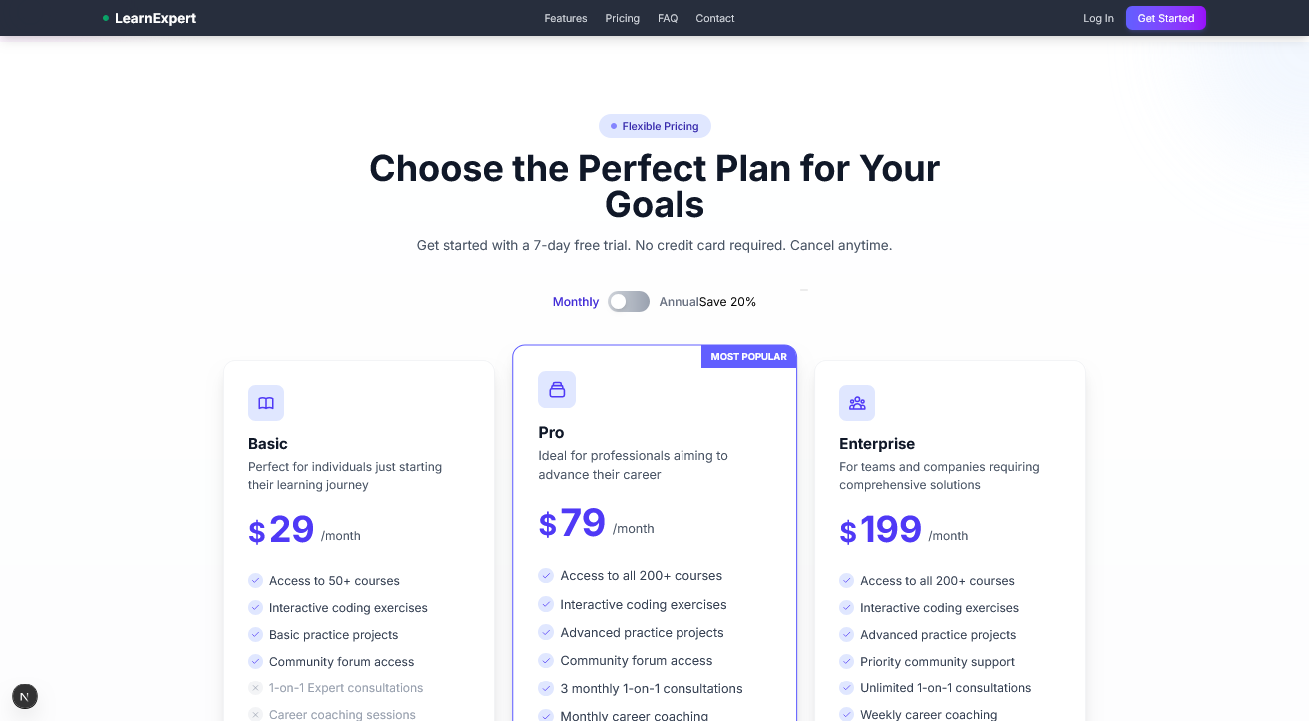
\includegraphics[width=0.9\textwidth,keepaspectratio]{week_2_img/payment_1.png}
  \caption{\textbf{Interface de paiement} pour les abonnements et services.}
  \label{fig:payment}
\end{figure}

Les fonctionnalités clés du système de paiement incluent :
\begin{itemize}
  \item Sélection de différentes formules d'abonnement
  \item Interface de saisie des informations de carte bancaire sécurisée
  \item Intégration avec un service de paiement externe (Stripe)
  \item Confirmation de paiement et génération de facture automatique
  \item Gestion des abonnements récurrents et des annulations
\end{itemize}

\section{Technologies Utilisées}

Pour le développement front-end de cette page d'accueil, les technologies suivantes ont été utilisées :
\begin{itemize}
  \item \textbf{Next.js :} Framework React pour le rendu côté serveur et la génération de sites statiques
  \item \textbf{Tailwind CSS :} Framework CSS utilitaire pour un design responsive et personnalisable
  \item \textbf{Framer Motion :} Bibliothèque d'animations pour ajouter des transitions et effets visuels
  \item \textbf{React Hook Form :} Gestion des formulaires avec validation
  \item \textbf{TypeScript :} Pour un code plus robuste avec typage statique
\end{itemize}

\section{Optimisations et Performances}

Une attention particulière a été portée à l'optimisation des performances :
\begin{itemize}
  \item Utilisation de l'optimisation d'images intégrée à Next.js
  \item Lazy loading des images et composants non critiques
  \item Minification du code CSS et JavaScript
  \item Mise en cache efficace pour réduire les temps de chargement
  \item Design responsive optimisé pour tous les appareils
\end{itemize}

\section{Méthodologie de Conception}

Le processus de conception de l'interface a suivi une approche méthodique :

\subsection{Analyse des Besoins et Recherche}
\begin{itemize}
  \item Étude des plateformes concurrentes pour identifier les meilleures pratiques
  \item Analyse des besoins des utilisateurs cibles
  \item Définition des objectifs principaux de la page d'accueil
\end{itemize}

\subsection{Wireframing et Prototypage}
\begin{itemize}
  \item Création de wireframes simples pour définir la structure de la page
  \item Développement de prototypes interactifs avec Figma
  \item Tests utilisateurs préliminaires pour valider les concepts
\end{itemize}

\subsection{Développement Itératif}
\begin{itemize}
  \item Implémentation progressive des différentes sections
  \item Sessions quotidiennes de feedback avec l'équipe
  \item Améliorations continues basées sur les retours
\end{itemize}

\section{Résultats et Impacts}

La conception de cette interface d'accueil a établi une base solide pour le développement des autres composants de la plateforme e-learning, en définissant une identité visuelle cohérente et en présentant clairement la proposition de valeur aux utilisateurs potentiels. 

\section{Conclusion}

Cette deuxième semaine de stage a été très productive, avec des avancées significatives dans le développement frontend de la plateforme. La création d'une page d'accueil attrayante et fonctionnelle constitue une étape importante du projet. Les différentes sections développées (Hero Section améliorée, Where We Are, fonctionnalités, FAQ, etc.) permettent de présenter efficacement la valeur ajoutée de la plateforme et d'inciter les utilisateurs à s'inscrire. Les prochaines étapes se concentreront sur le développement des interfaces internes pour les utilisateurs connectés et l'intégration des fonctionnalités backend. 

% Week 3 content
\chapter{Semaine 3 : Développement des Interfaces Utilisateur et Traitement des Données}
\thispagestyle{fancy}

La troisième semaine du stage a été consacrée au développement des interfaces utilisateur pour la plateforme d'apprentissage en ligne, ainsi qu'à la mise en place d'un système avancé de traitement des données de contenu. Ces avancées ont permis de construire les fondations interactives de la plateforme et d'optimiser le traitement des ressources pédagogiques.

\section{Intégration et Déploiement de la Base de Données}

La première tâche de cette semaine a été de structurer et pérenniser les données collectées lors des phases précédentes du projet.

\subsection{Collecte et Préparation des Données}

La semaine a débuté par la finalisation du processus de web scraping initié précédemment. Ce processus a permis de collecter un volume important de données éducatives provenant principalement de W3Schools. Les données brutes ont ensuite été soumises à un nettoyage préliminaire pour éliminer les éléments non pertinents et standardiser les formats.

\subsection{Transfert des Données vers MongoDB}

Les fichiers JSON contenant les données scrappées et préalablement nettoyées ont été migrés vers une base de données MongoDB. Chaque type de contenu a été organisé dans des collections distinctes, créant ainsi une structure cohérente et facilement interrogeable.

\begin{figure}[h!]
  \centering
  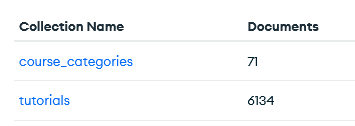
\includegraphics[width=0.9\textwidth,keepaspectratio]{week_3_img/Screenshot 2025-05-19 234047.png}
  \caption{\textbf{Interface MongoDB Atlas} montrant les différentes collections de données.}
  \label{fig:mongodb_collections}
\end{figure}

\subsection{Déploiement Cloud sur MongoDB Atlas}

Pour assurer une accessibilité optimale et une scalabilité future, la base de données a été déployée sur MongoDB Atlas, une plateforme de base de données en tant que service (DBaaS). Cette solution cloud offre plusieurs avantages :

\begin{itemize}
  \item Haute disponibilité avec réplication automatique
  \item Surveillance en temps réel des performances
  \item Sauvegardes automatisées
  \item Sécurité renforcée avec authentification et chiffrement
  \item Scalabilité horizontale et verticale selon les besoins
\end{itemize}

\subsection{Connexion de l'Application à la Base de Données}

Une fois la base de données déployée, la connexion entre l'application backend et l'instance MongoDB hébergée sur Atlas a été établie. Cette étape cruciale a permis d'assurer que l'application puisse lire et écrire des données de manière fiable et sécurisée.

\subsection{Évolution vers une Solution JSON Locale}

Après des tests approfondis, une décision stratégique a été prise de migrer d'une architecture MongoDB vers une solution basée sur des fichiers JSON locaux. Cette transition a été motivée par :

\begin{itemize}
  \item La réduction de la complexité architecturale pour la phase actuelle du projet
  \item L'amélioration de l'expérience de développement avec un accès direct aux données
  \item La compatibilité optimale avec le framework Next.js et ses capacités de rendu côté serveur
  \item La simplification du déploiement et de la maintenance pour les premiers stades du projet
\end{itemize}

Cette migration a nécessité l'adaptation des modèles de données et le développement d'une nouvelle logique d'accès aux données, mais a considérablement simplifié le processus de développement.

\section{Conception et Développement de l'Interface Utilisateur}

Après avoir développé la page d'accueil la semaine précédente, l'accent a été mis sur la création des interfaces principales que les utilisateurs utiliseront quotidiennement pour accéder aux contenus et suivre leur progression.

\subsection{Interface d'Accueil des Utilisateurs Connectés}

Une interface d'accueil spécifique pour les utilisateurs connectés a été développée, offrant un accès rapide aux cours en cours, aux recommandations personnalisées et aux dernières activités.

\begin{figure}[h!]
  \centering
  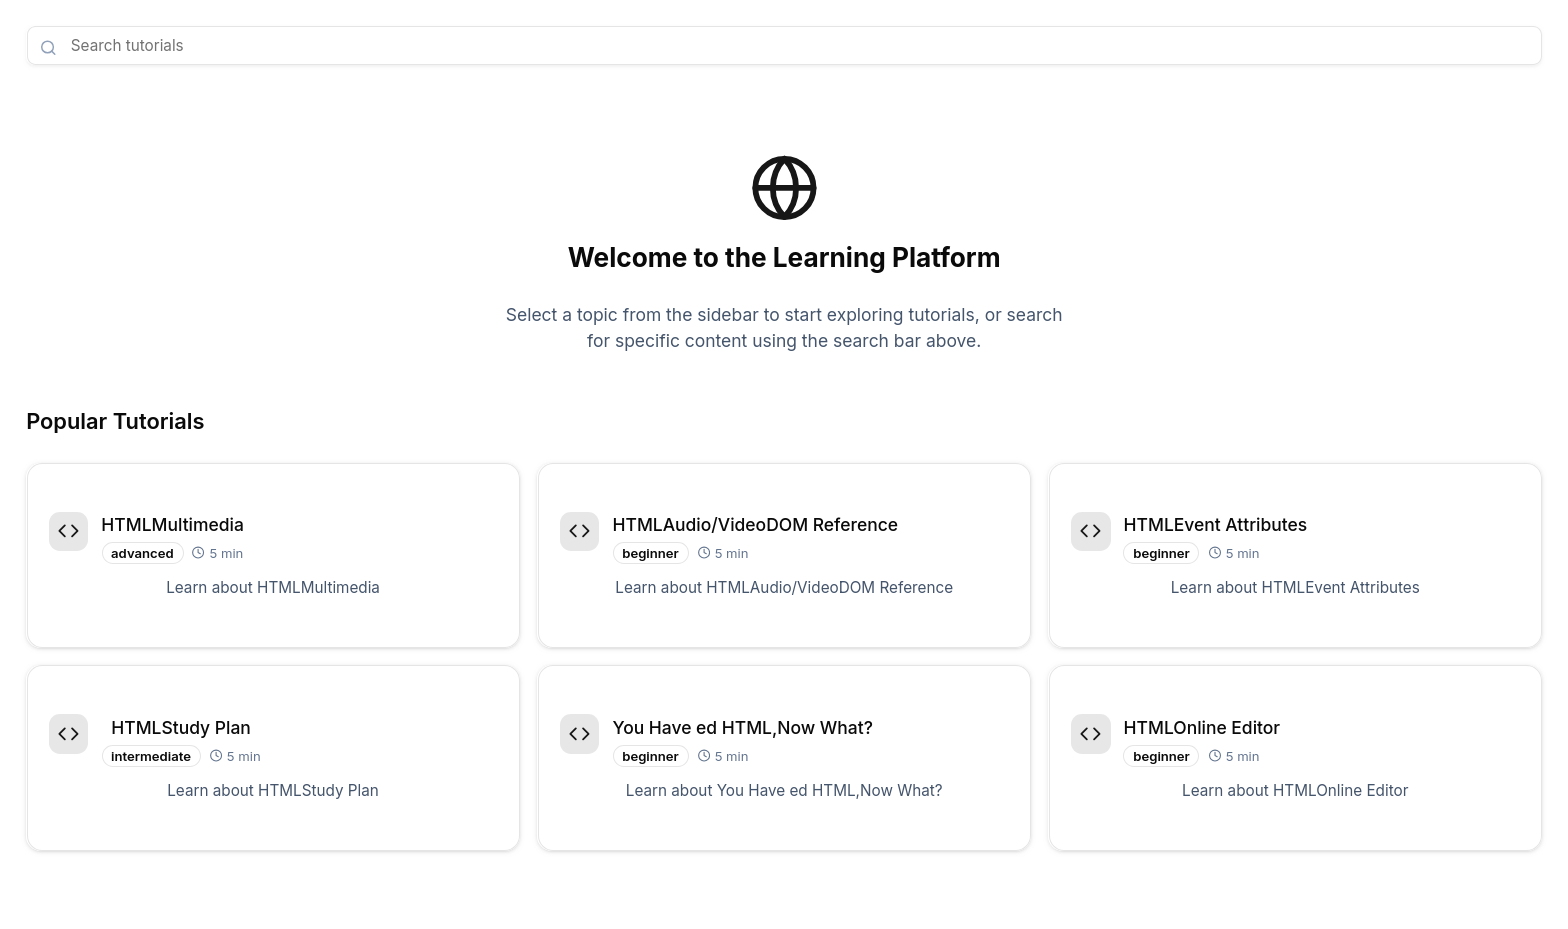
\includegraphics[width=0.9\textwidth,keepaspectratio]{week_3_img/accueil.png}
  \caption{\textbf{Interface d'accueil personnalisée} pour les utilisateurs connectés.}
  \label{fig:user_dashboard}
\end{figure}

\subsection{Barre Latérale de Navigation}

Une barre latérale de navigation intuitive a été implémentée pour faciliter l'accès aux différentes sections de la plateforme.

\begin{figure}[h!]
  \centering
  
\includegraphics[width=0.4\textwidth,keepaspectratio]{week_3_img/sidebare.png}
  \caption{\textbf{Barre latérale de navigation} avec accès aux principales fonctionnalités.}
  \label{fig:sidebar_nav}
\end{figure}

Cette barre latérale comprend :
\begin{itemize}
  \item Accès au tableau de bord personnel
  \item Catalogue de cours et formations
  \item Suivi de progression
  \item Calendrier des sessions de consultation
  \item Paramètres du compte
  \item Centre de notifications
\end{itemize}

\subsection{Interface de Consultation des Cours}

L'interface de consultation des cours a été conçue pour offrir une expérience d'apprentissage immersive et efficace.

\begin{figure}[h!]
  \centering
  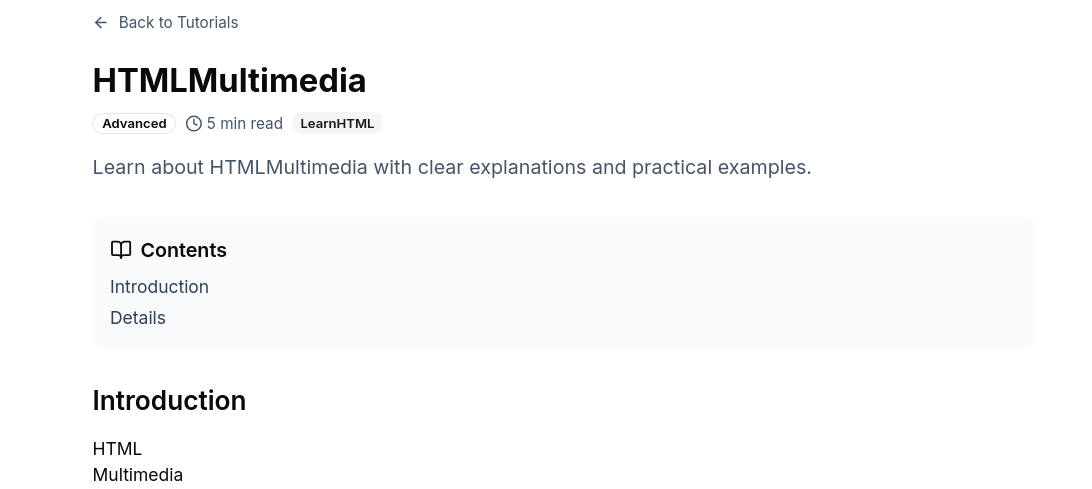
\includegraphics[width=0.9\textwidth,keepaspectratio]{week_3_img/part1.png}
  \caption{\textbf{Interface de consultation des cours} - Partie théorique.}
  \label{fig:course_view_part1}
\end{figure}

\begin{figure}[h!]
  \centering
  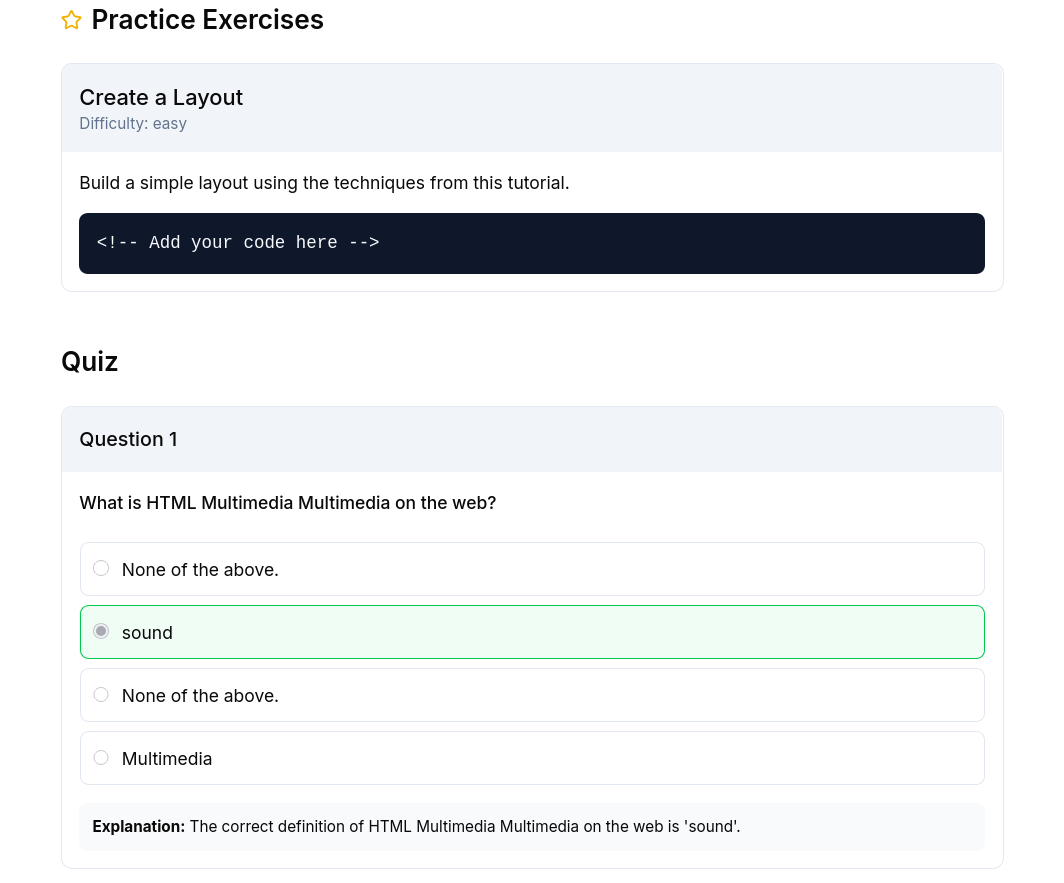
\includegraphics[width=0.9\textwidth,keepaspectratio]{week_3_img/part2.png}
  \caption{\textbf{Interface de consultation des cours} - Partie pratique avec exercices interactifs.}
  \label{fig:course_view_part2}
\end{figure}

Les caractéristiques principales de cette interface incluent :
\begin{itemize}
  \item Affichage clair du contenu théorique avec mise en forme optimisée
  \item Navigation intuitive entre les différentes sections du cours
  \item Exercices interactifs intégrés directement dans l'interface
  \item Suivi de progression en temps réel
  \item Possibilité de prendre des notes contextuelles
  \item Mode sombre/clair pour améliorer le confort de lecture
\end{itemize}

\section{Traitement Avancé des Données de Contenu}

Une partie importante de cette semaine a été consacrée à l'optimisation du traitement des données de contenu éducatif.

\subsection{Défis du Traitement des Données}

Le traitement des données collectées présentait plusieurs défis :
\begin{itemize}
  \item Distinction entre le contenu textuel explicatif et les exemples de code
  \item Structuration cohérente des exemples et exercices
  \item Préservation des formatages spécifiques (tableaux, listes, etc.)
  \item Gestion des caractères spéciaux et encodages
  \item Extraction des métadonnées pertinentes
\end{itemize}

\subsection{Problématique du Scraping et Nettoyage des Données}

L'un des défis majeurs rencontrés a été la séparation du contenu textuel explicatif et des extraits de code dans les sections détaillées des cours. Plusieurs approches ont été explorées :

\begin{itemize}
  \item Tentatives initiales avec des expressions régulières et des algorithmes de traitement de texte, atteignant une précision maximale de 80\%
  \item Expérimentation avec un agent IA basé sur des modèles de langage large (LLM) pour effectuer cette séparation de manière plus intelligente
  \item Découverte finale que la structure HTML particulière de W3Schools nécessitait une approche de scraping spécifique
\end{itemize}

La solution définitive a impliqué une refonte du script de scraping pour mieux cibler les éléments HTML spécifiques, permettant ainsi d'obtenir des données brutes de meilleure qualité dès le départ.

\subsection{Implémentation d'un Pipeline de Traitement LLM}

Pour surmonter ces défis, un pipeline de traitement basé sur des modèles de langage large (LLM) a été conçu et implémenté.

\begin{figure}[h!]
  \centering
  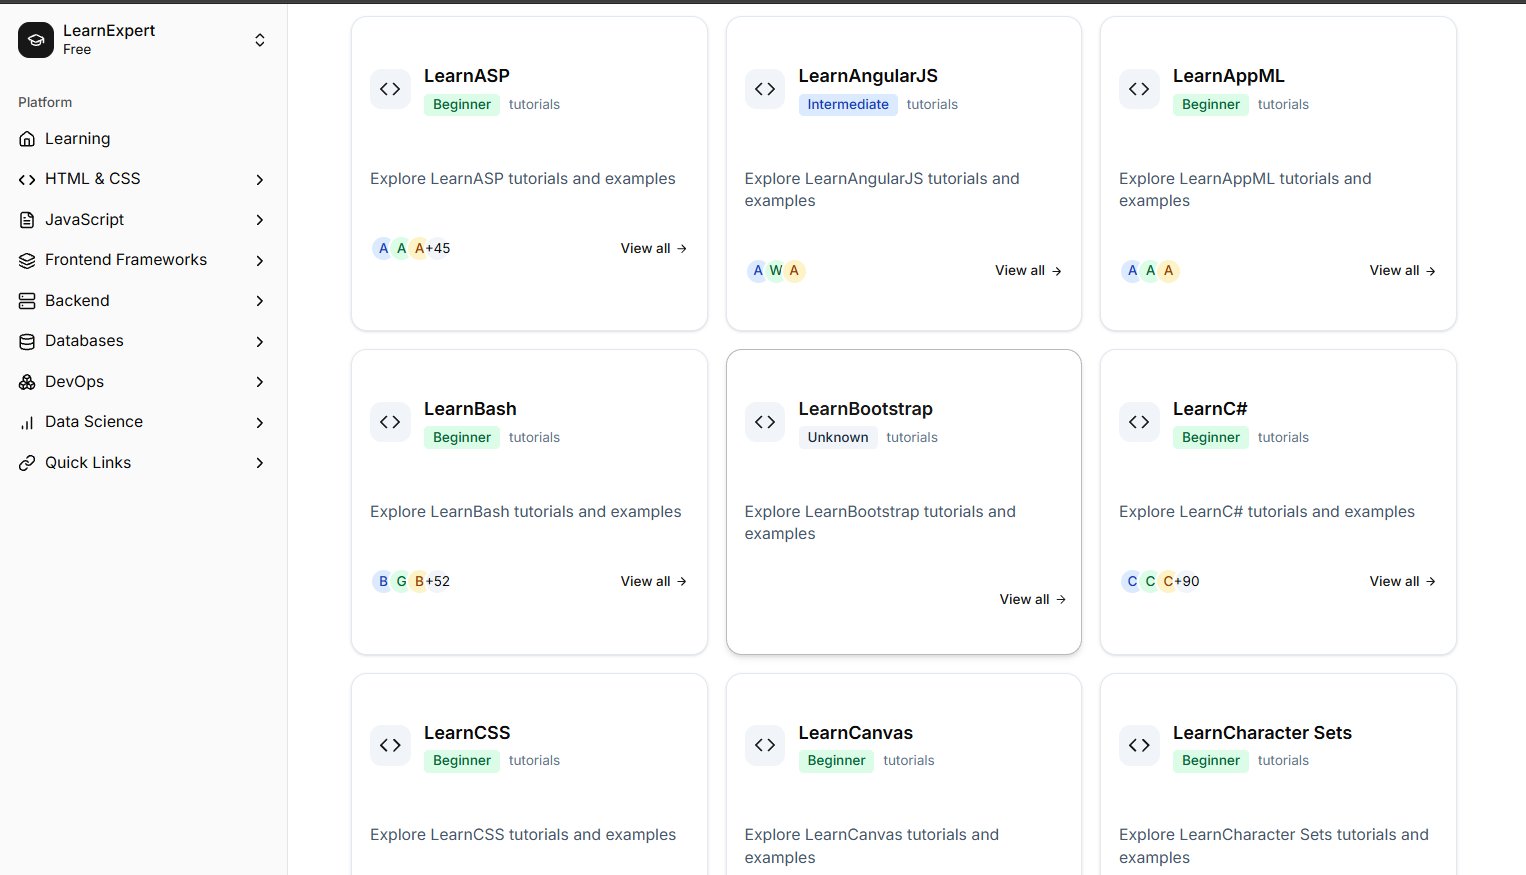
\includegraphics[width=0.9\textwidth,keepaspectratio]{week_3_img/Screenshot 2025-05-20 164411.png}
  \caption{\textbf{Interface d'administration du pipeline LLM} montrant les statistiques de traitement.}
  \label{fig:llm_pipeline}
\end{figure}

\subsection{Stratégie d'Optimisation Multi-LLM}

Le traitement initial utilisant un LLM unique ayant démontré une excellente précision mais des performances limitées en termes de vitesse, une stratégie d'optimisation a été mise en place :

\begin{itemize}
  \item \textbf{Utilisation simultanée de plusieurs fournisseurs LLM :} Parallélisation des requêtes vers différentes API
  \item \textbf{Traitement asynchrone :} Optimisation de la latence perçue en traitant plusieurs segments de données simultanément
  \item \textbf{Segmentation intelligente :} Division des données en unités de traitement optimales pour chaque type de modèle
  \item \textbf{Gestion des requêtes :} Assignation statique de segments spécifiques à des modèles dédiés pour simplifier la gestion de la concurrence
\end{itemize}

Cette approche a permis de réduire significativement le temps de traitement tout en maintenant une qualité optimale, passant d'environ 15 heures à 7-8 heures pour l'ensemble des données.

\section{Intégration Frontend-Backend}

Une attention particulière a été portée à l'intégration efficace entre le frontend et le backend de la plateforme.

\subsection{Développement des Routes d'API}

Des routes d'API RESTful ont été développées pour permettre à l'interface utilisateur d'accéder aux données structurées dans MongoDB :

\begin{itemize}
  \item Routes d'authentification et de gestion des utilisateurs
  \item Routes d'accès au catalogue de cours
  \item Routes de suivi de progression
  \item Routes de gestion des consultations et réservations
  \item Routes d'analytics et de rapports
\end{itemize}

\subsection{Optimisation des Requêtes}

Les requêtes MongoDB ont été optimisées pour garantir des performances optimales :

\begin{itemize}
  \item Création d'index appropriés pour accélérer les recherches fréquentes
  \item Limitation des champs retournés aux données strictement nécessaires
  \item Utilisation de projections pour alléger les transferts de données
  \item Mise en place de pagination pour les listes volumineuses
  \item Implémentation de mécanismes de mise en cache pour les données fréquemment consultées
\end{itemize}

\subsection{Adaptation à l'Architecture JSON}

Suite à la migration vers des fichiers JSON locaux, l'architecture d'accès aux données a été adaptée :

\begin{itemize}
  \item Développement de fonctions de récupération (fetch) optimisées pour les fichiers JSON
  \item Mise en place d'un système de chargement dynamique des données pour les différentes sections de l'interface
  \item Intégration des capacités de rendu côté serveur de Next.js pour améliorer les performances
\end{itemize}

Cette adaptation a permis de maintenir toutes les fonctionnalités prévues tout en simplifiant l'architecture globale du système.

\section{Tests et Validation}

Pour garantir la qualité et la fiabilité des interfaces et systèmes développés, plusieurs types de tests ont été mis en place :

\subsection{Tests d'Interface Utilisateur}

\begin{itemize}
  \item \textbf{Tests de compatibilité :} Vérification du rendu sur différents navigateurs (Chrome, Firefox, Safari, Edge)
  \item \textbf{Tests de responsive design :} Validation de l'adaptation aux différentes tailles d'écran
  \item \textbf{Tests d'accessibilité :} Conformité aux standards WCAG pour garantir l'inclusivité
  \item \textbf{Tests d'utilisabilité :} Évaluation de l'intuitivité et de la fluidité de navigation
\end{itemize}

\subsection{Tests Fonctionnels et d'Intégration}

\begin{itemize}
  \item \textbf{Tests des routes d'API :} Validation des entrées/sorties et gestion des erreurs
  \item \textbf{Tests d'intégration :} Vérification de la communication correcte entre frontend et backend
  \item \textbf{Tests de performance :} Mesure des temps de réponse et optimisation des goulots d'étranglement
  \item \textbf{Tests de charge :} Simulation d'utilisation intensive pour évaluer la robustesse
\end{itemize}

\subsection{Planification Stratégique pour l'Avenir}

En fin de semaine, une réflexion stratégique a été menée concernant l'enrichissement du contenu et la différenciation de la plateforme :

\begin{itemize}
  \item Identification du besoin de diversifier les sources de contenu au-delà de W3Schools
  \item Planification de l'intégration d'éléments interactifs avancés, comme un éditeur de code basé sur les technologies VSCode
  \item Initiation à l'apprentissage des techniques d'optimisation pour les moteurs de recherche (SEO) pour améliorer la visibilité future de la plateforme
\end{itemize}

\section{Conclusion}

Cette troisième semaine a marqué des avancées significatives dans le développement de la plateforme e-learning. La mise en place d'interfaces utilisateur intuitives et ergonomiques, couplée à un système sophistiqué de traitement des données éducatives, a permis de poser les fondations solides pour l'expérience utilisateur finale. L'utilisation innovante de technologies comme MongoDB Atlas et les modèles de langage large (LLM) a apporté des solutions efficaces aux défis techniques rencontrés.

Les interfaces développées durant cette semaine offrent maintenant aux utilisateurs un environnement d'apprentissage fluide et immersif, tandis que l'optimisation du traitement des données garantit une qualité exceptionnelle du contenu éducatif proposé. Les décisions stratégiques prises, notamment la simplification de l'architecture de données et la planification d'éléments différenciateurs, posent les bases d'une plateforme compétitive et évolutive. 

% Week 4 content
\chapter{Semaine 4 : Finalisation, Tests et Déploiement}
\thispagestyle{fancy}
 
Contenu de la semaine 4 à venir. Cette section sera complétée ultérieurement. 

\chapter{Conclusion et Perspectives}
\thispagestyle{fancy}

Ce stage de quatre semaines chez LearnTech Solutions m'a permis de participer activement au développement d'une plateforme e-learning innovante. Au cours de cette période, j'ai pu mettre en pratique mes connaissances théoriques et acquérir de nouvelles compétences techniques dans un environnement professionnel stimulant.

\section{Synthèse des Réalisations}

Durant ces quatre semaines, les principales réalisations ont été :
\begin{itemize}
  \item La conception de l'architecture microservices pour la plateforme
  \item La participation au développement des interfaces utilisateur
  \item L'implémentation de systèmes de traitement et nettoyage de données
  \item La contribution à l'optimisation des performances et à l'amélioration de l'expérience utilisateur
\end{itemize}

\section{Compétences Acquises}

Ce stage m'a permis de développer de nombreuses compétences :
\begin{itemize}
  \item \textbf{Compétences techniques :} Approfondissement des connaissances en développement web moderne (Next.js, API REST), en architecture microservices et en traitement de données avec des modèles LLM
  \item \textbf{Compétences méthodologiques :} Maîtrise des outils de gestion de projet agile, de versionnement et de déploiement continu
  \item \textbf{Compétences transversales :} Amélioration des capacités de communication, de travail en équipe et d'adaptation à un environnement professionnel
\end{itemize}

\section{Perspectives}

Ce projet ouvre plusieurs perspectives intéressantes :
\begin{itemize}
  \item \textbf{Pour l'entreprise :} Finalisation et commercialisation de la plateforme e-learning, avec des fonctionnalités supplémentaires comme l'intelligence artificielle pour la personnalisation des parcours d'apprentissage
  \item \textbf{Pour ma carrière :} Approfondissement des compétences en développement full-stack et en architecture de systèmes complexes
\end{itemize}

En conclusion, ce stage a été une expérience extrêmement enrichissante qui m'a permis d'approfondir mes connaissances techniques tout en développant ma compréhension des enjeux liés au développement de solutions éducatives numériques. Les compétences acquises et l'expérience professionnelle seront des atouts précieux pour ma future carrière.

\appendix
\chapter{Annexes}
\thispagestyle{fancy}
[Diagrammes UML, exemples de code, captures d'écran de l'interface]

\end{document}
